
\documentclass[conference]{IEEEtran}
%\usepackage{draftwatermark} \SetWatermarkLightness{ 0.9 } \SetWatermarkScale{ 1 } \SetWatermarkText{DRAFT}
\usepackage[utf8]{inputenc}
\usepackage{amsmath}
\usepackage{amssymb}
\usepackage{color}
\usepackage{verbatim}
\usepackage{fancyhdr}
\usepackage[hidelinks]{hyperref} 


\newcommand{\Fp}{\mathbb{Z}_p}
\newcommand{\sk}{\texttt{sk}}
\newcommand{\pk}{\texttt{pk}}
\newcommand{\id}{\texttt{id}}
\newcommand{\seed}{\texttt{seed}}
\newcommand{\ind}{\texttt{index}}
\newcommand{\out}{\texttt{output}}
\newcommand{\cmt}{\texttt{commit}}

\newcommand{\Alloc}{\textsc{Alloc}}
\newcommand{\mask}{\textsc{mask}}
\newcommand{\func}{\textsc{func}}
\newcommand{\hash}{\textsc{hash}}


\usepackage{pgf,tikz}
\usepackage{scrextend}
\usepackage{mathrsfs}
\usepackage{cite}
\usetikzlibrary{arrows}

\title{Autonomys: Foundation Layer for AI3.0}

\author{Chen Feng$^{1,}$$^{2}$, Dariia Porechna$^{3}$, Jeremiah Wagstaff$^{1,}$$^{3}$\\
$^1$Autonomys Labs\\
$^2$University of British Columbia\\
$^3$Subspace Foundation\\


\thanks{The authors are listed in alphabetical order.}}

\IEEEoverridecommandlockouts % using \thanks{}

\begin{document}
\pagestyle{plain}
\fancyhf{}
\cfoot{\thepage}
\maketitle
\begin{abstract}
As we approach the widespread integration of artificial intelligence (AI) into our everyday lives, we face a pivotal moment of redefinition for our traditional understanding of the role of human and machine agency in contemporary society. AI technologies present both significant challenges to prevailing socioeconomic structures and theory, and unprecedented opportunities for the establishment of novel paradigms. Autonomys offers a vision of an AI-augmented world that enhances human autonomy rather than diminishing it. The Autonomys Network—our decentralized infrastructure stack for secure, self-sovereign human-AI collaboration—requires only an SSD to join. We have built the network from first principles to simultaneously achieve security, scalability, and decentralization based on original multi-year research. At its core, the Autonomys Network implements Subspace, a novel storage-based consensus protocol that decouples consensus from execution. This proposer-builder separation allows the Autonomys Network to independently scale transaction throughput and storage requirements while maintaining a fully decentralized blockchain with a low barrier to participation—all vital for the realization of decentralized AI—or AI3.0.
\end{abstract}

\section{Background}

The rapid advancement of artificial intelligence (AI) technologies is ushering in a new era of socioeconomic transformation. Recent breakthroughs in machine learning (ML), particularly in deep learning and natural language processing, have led to AI systems capable of performing tasks once thought to be the exclusive domain of human intelligence\cite{lecun2015}. This progress has sparked debates about the future of work, with some experts predicting widespread job displacement\cite{frey2017}, and others envisioning new forms of human-AI collaboration\cite{brynjolfsson2014}. Concurrently, the rise of blockchain technology has introduced novel paradigms for decentralized systems and digital identity\cite{zheng2017}. These technological developments have occurred against a backdrop of growing concerns about data privacy, algorithmic bias, and the concentration of AI capabilities in the hands of a few large corporations\cite{oneil2016}. As we approach the potential development of Artificial General Intelligence (AGI) and Artificial Superintelligence (ASI)—when AI reaches and then exceeds human intelligence\cite{bostrom2014}—it becomes imperative to establish frameworks that ensure AI systems align with human values and preserve human autonomy in an increasingly automated world\cite{russell2019}. The Autonomys Network proposes and seeks to implement a new paradigm of \textit{radical autonomy}, or absolute digital self-governance.

\section{AI3.0}

The evolution of AI can be categorized into three broad phases, each characterized by a unique relationship between humans, decentralization, and AI:
\begin{itemize}
    \item \textit{\textbf{AI1.0}} | Centralized ML: Deep learning becomes widespread as developers are able to build models with the likes of TensorFlow and PyTorch running on cloud computing provided by Big Tech. Humans are primarily passive consumers of AI technologies, interacting with narrow, rule-based systems designed for specific tasks.
    \item \textit{\textbf{AI2.0}} | Centralized Generative AI: Large language models (LLMs), such as ChatGPT, Gemini, and Claude, emerge alongside other Generative AI technologies built by Big Tech. Humans are offered more interactive AI experiences, albeit still through platforms controlled and deployed by centralized entities.
    \item \textit{\textbf{AI3.0}} | Decentralized Human-centric AI: Open, accessible and collaborative web3-enabled AI model, app and agent development and deployment. Decentralization ensures a transparent, composable, and secure ecosystem where innovation thrives. Humans not only interact with AI, but customize, train and deploy their own highly personalized Autonomys agents to act on their behalf, blurring the boundary between AI creator and consumer. The Age of Autonomy is the culmination of this paradigm.
    \end{itemize} 

\section{Age of Autonomy}

Throughout the history of technological development, humanity has consistently striven for the same fundamental needs to be fulfilled: \textit{safety}, including both physical and resource security; \textit{connection}, be it physical or emotional, to fellow humans or cultural collectives; and \textit{prosperity}, through self-improvement and socioeconomic development. Many experts have discussed AI's impact on human safety, connection and prosperity \cite{brynjolfsson2014} \cite{russell2019} \cite{miessler}. Autonomys is using these three fundamental human desires as guiding principles to propose a human-centric vision of a post-AI-revolution future.

In today's world, one's safety and prosperity are mediated largely by one's access to economic resources. As job security becomes progressively more threatened by the advent of sophisticated AI\cite{frey2017}, we should evolve our contemporary economic systems with continued human relevance and agency in mind. This can be achieved through widening global access to permissionless incentivized contribution networks, and by augmenting human capabilities with personal AI agents that seamlessly interact and collaborate in a verifiable way—all free of centralized control.

The trajectory of AI development is trending towards the training and running of smaller, specialized AI models on personal edge devices. When integrated into every action taken on a personal device \cite{apple}, these AI will have the context of all knowledge about the device's owner, including past and present interactions with other people or services; personal preferences in entertainment, food, clothing and partners; health metrics; financial statements; political allegiances; and everything else that has ever gone through the device. Coupling access to complete contextual data with agentic capabilities transforms personal AI into personal agents that can represent you online and act on your behalf—booking medical visits and vacations, ordering groceries, coordinating meetings, managing money, or participating in governance. Crucially, personal agents will be able to analyze and filter the endless information streams around us—insurmountable for a single person to process—aiding in our decision-making.

It is prudent to estimate the emergence of at least as many agents online as there are smartphones. Practically, we can expect each person and business to have multiple specialized AI representatives. This global mesh of billions of agents will communicate and exchange funds with each other online and with service providers via agent-specific permissioned actions. Humans and agents will need to be able to verify whether the AI they are interacting with within this autonomous agent economy is truthfully representing themselves as agents of particular individuals or organizations (see \href{sec:agentids}{\textit{Identity for Agents}}).

The Autonomys-facilitated agent economy will foster a rich ecosystem of human and AI collaboration. Autonomys' development platform will provide cutting-edge tools for individuals and organizations to train and deploy agents, acquire highly valuable technological skills, and amplify their potential. Autonomys agents will be able to exchange mutual authorizations via blockchain to provide real-world goods and services, while humans maintain oversight of and control over them. This dynamic creates new avenues for entrepreneurship and value generation as individuals and organizations leverage AI capabilities to augment their own skills and offerings. Autonomys' vision preserves humanity's economic relevance by emphasizing domains where the unique human capacity for creativity, emotional intelligence, and complex problem-solving has not been replicated by AI.

In contrast to predicted futures populated by a universal basic income (UBI)-dependent humanity\cite{altman2021} subject to a diminished human agency and economic relevance, Autonomys champions radical autonomy through incentivized participation and contribution to a self-sustaining ecosystem, inspired by Ethereum's pioneering model. We recognize human potential as a dynamic force that can be continually expanded through education, technological integration, and innovative socioeconomic systems.

By empowering individuals with self-sovereign digital identities, control over their data assets, and tools for safe AI collaboration, Autonomys is forging a future where humans and AI coexist productively and harmoniously. This new paradigm not only preserves human economic relevance but amplifies our collective potential, ushering in an era of unprecedented innovation, creativity, and shared prosperity.

\section{Autonomys AI3.0 Stack}

The Autonomys Network serves as the technological infrastructure for this paradigm shift, providing a verticalized decentralized AI stack encompassing (Fig.\,\ref{fig:stack}):
\begin{figure}
    \centering
    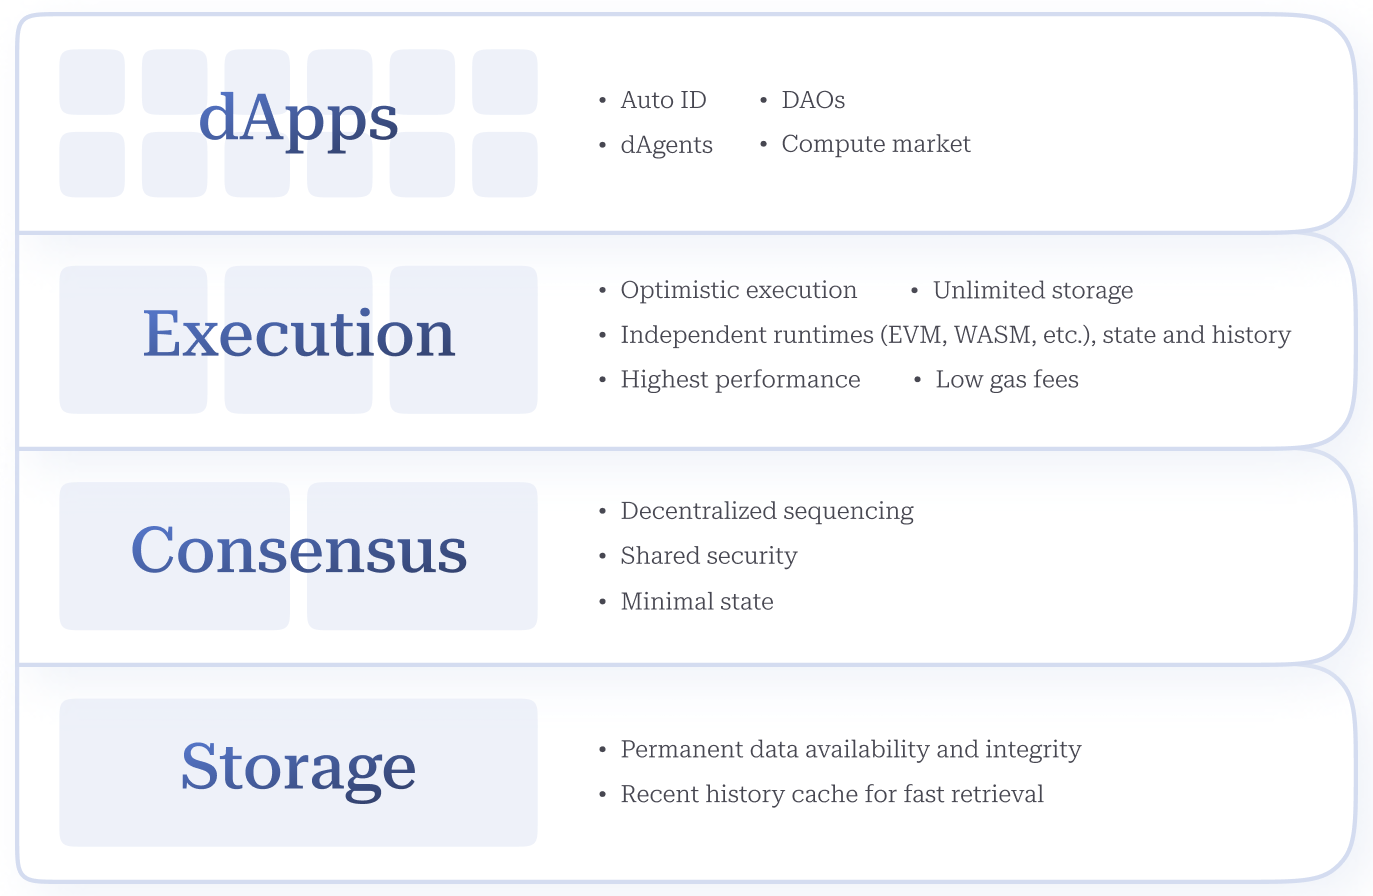
\includegraphics[width=1\linewidth]{ai30_stack.png}
 \caption{Autonomys Network stack}
 \label{fig:stack}
\end{figure}
\begin{itemize}
    \item \textit{\textbf{dApp/Agent Layer}}: facilitating the development and deployment of super dApps (AI-powered dApps) and Autonomys agents (Auto ID-integrated on-chain agents) for verifiable digital interaction. 
    \item \textit{\textbf{Execution/Domain Layer}}: secure, scalable distributed computing for AI training, inference and agentic workflows.
    \item \textit{\textbf{Consensus Layer}}: verifiable decentralized sequencing and transaction validation for shared security.
    \item \textit{\textbf{Storage Layer}}: distributed storage ensures data integrity and permanent availability—crucial for storing vast amounts of AI data.
\end{itemize}

Utilizing the \hyperref[sec:subspace]{Subspace Protocol}~\cite{subspacev1}, with its innovative \hyperref[sec:poas]{Proof-of-Archival-Storage} (PoAS) consensus mechanism~\cite{subspacev2}, our decentralized physical infrastructure network (DePIN) incentivizes active participation through the permissionless contribution of any amount of storage space or compute, or staking of any amount of tokens, permitting unprecedented accessibility.

%Ultimately, Autonomys is dedicated to building an ecosystem where every human has many powerful, automatically interoperable, personally aligned models at their disposal. The three main steps on the path towards this collaborative ecosystem are AI-powered dApps, new agent coordination mechanisms, and ownership and governance. The Autonomys Network provides the infrastructure to achieve all three in a decentralized, scalable and verifiable way on-chain, adhering to the outlined vision roadmap:

%Data Storage → Data Provenance → Data Economy → Networks of agents → Age of Autonomy.

\subsection{Future-Proofing Storage for AI3.0}

The advent of AI3.0 brings with it an unprecedented demand for vast, permanent decentralized storage capable of rapid data retrieval. As AI systems become more sophisticated and personalized, they require access to enormous datasets for training, fine-tuning, and real-time decision-making. Traditional centralized storage systems are ill-equipped to handle the scalability, security and accessibility requirements of this new paradigm.

Decentralized storage solutions offer several key advantages: ensuring data integrity and availability through redundancy; mitigating single points of failure; and allowing for a more equitable distribution of resources. Moreover, the permanence of data storage is crucial for maintaining historical records, enabling long-term learning, and supporting accountability in AI decision-making processes. Rapid data retrieval is equally essential, as AI3.0 agents must be able to access relevant information swiftly to provide real-time responses and make informed decisions. This combination of vast capacity, permanence, decentralization, and speed is fundamental to realizing the full potential of AI3.0—where personalized Autonomys agents operate efficiently and verifiably at scale.

Autonomys addresses this growing demand via our super-fast, hyper-scalable, permanent distributed storage network (DSN) and content-delivery network (CDN) supported by multiple reliability layers (see \href{sec:dsn}{\textit{Distributed Storage}}); secured by PoAS consensus; and served by thousands of easy-to-setup nodes worldwide. At the core of the Autonomys economy is the concept of data sovereignty, enabled by our vast decentralized storage and systems for content contribution, provenance, and compensation. This revolutionary approach to understanding and managing personal information and intellectual property—where individuals retain control over their data assets and can opt to monetize them for AI training and optimization purposes—pioneers a novel economic model where humans may choose to share their personal data and receive fair compensation for the value their data provides in enhancing AI systems, rather than having their information exploited without remuneration, as is currently the case.

\subsection{Content Provenance and Data Sovereignty}

Data sovereignty—the ability of individuals to control and maintain authority over their personal data and digital presence—is crucial in an era where sensitive data is frequently exploited by criminal actors and centralized entities. Data sovereignty cannot be achieved without a way to establish ownership and provenance of data in a verifiable way.

Cryptographically linking digital content with its creator's authenticated identity establishes an immutable record of the origin and subsequent modifications \cite{hasan2009}. Such a system empowers users with granular control over their data-sharing preferences and provides a robust framework for verifying the authenticity of digital assets. It also offers a potential solution to the challenges posed by synthetic media, allowing recipients to discern between genuine and artificially generated content \cite{westerlund2019}. Furthermore, as AI systems continue to evolve and generate increasingly sophisticated outputs, the ability to trace the lineage of training data and resultant content is becoming increasingly important \cite{brundage2020}.

\subsection{Digital Identity}

Autonomys' secure protocol for the provision of decentralized digital identities—Autonomys Identity (Auto ID)—simultaneously allows for the authentication of AI-generated content and permissioning of agentic actions. Utilizing advanced cryptographic techniques, our robust self-sovereign identity (SSI) framework (deployed as a registered runtime on Autonomys' domain layer) enables individuals to verify their identity without resorting to invasive biometric procedures. This foundation of digital trust is crucial for facilitating economic collaboration between humans and AI.

Key properties of the Auto ID system include:
\begin{itemize}
    \item \textit{Self-sovereignty}: Users maintain complete control over their digital identity, with autonomy in information-sharing decisions via a combination of encryption, zero-knowledge and verifiable credentials.
    \item \textit{Verifiability}: Cryptographic proofs ensure the authenticity of claims without compromising personal information.
    \item \textit{Universality}: Auto IDs can be issued to any entity, human or artificial, enabling a common identity standard across the digital ecosystem.
    \item \textit{Versatility}: The Auto ID framework supports identity self-issuance, issuance by another entity, and co-issuance by multiple entities.
    \item \textit{Interoperability}: Auto ID is designed for seamless integration with existing identity systems such as X.509 \cite{rfc5280} and Decentralized Identifiers \cite{did-core}.
\end{itemize}

Auto ID plays a crucial role in establishing content provenance and ensuring data sovereignty. After obtaining an Auto ID, entities can digitally sign the content they produce, establishing a verifiable and tamper-proof record of authenticity and provenance for data, linked with their Auto ID. This is particularly important as the line between human-created and machine-generated content becomes increasingly blurred.

Cryptographically linking digital content with its creator's authenticated identity establishes an immutable record of origin and subsequent modifications. Such a system empowers users with granular control over their data-sharing preferences and provides a robust framework for verifying the authenticity of digital assets. It also offers a potential solution to the challenges posed by synthetic media, allowing recipients to discern between genuine and artificially generated content.

Autonomys also offers the ability to attach cryptographic identity claims to an Auto ID via verifiable credentials. For example, an individual may attach a verifiable credential to their Auto ID showing they have a valid diploma, and later utilize that claim when a diploma is required.

\subsection{Proof-of-Personhood}

As we transition into an agent-integrated world, the ability to distinguish between humans and artificial entities becomes increasingly crucial. Auto ID implements proof-of-personhood (PoP) via our composable, probabilistic PoP protocol Auto Score. This system is designed to address the growing need for verifiable human identity in digital spaces, particularly in scenarios where AI agents and humans interact seamlessly.

A strong PoP system is important in the AI3.0 era for several reasons:

\begin{itemize}
    \item \textit{Preventing AI Impersonation}: As AI becomes more sophisticated, the risk of AI systems impersonating humans increases. A strong PoP system helps maintain the integrity of human-to-human interactions in digital spaces.
    \item \textit{Ensuring Fair Resource Distribution}: In a world where AI agents could potentially overwhelm systems, PoP ensures that resources and opportunities are fairly distributed among genuine human users.
    \item \textit{Maintaining Democratic Processes}: For online voting or governance systems, PoP is crucial to prevent manipulation by automated systems or sock puppet accounts.
    \item \textit{Preserving Human-Centric Economies}: As AI agents become more prevalent in economic systems, PoP helps maintain spaces for human economic activity and prevents AI from dominating marketplaces.
    \item \textit{Ethical AI Development}: PoP systems can help ensure that AI training data comes from verified human sources, promoting more ethical and representative AI development.
\end{itemize}

Auto Score leverages pre-existing evidence of personhood and zero-knowledge proofs (ZKPs) to generate privacy-preserving, verifiable credentials that combine to offer a probabilistic proof-of-personhood score. Supporting ZKP-secured e-passport verification as a primary personhood factor, users need only scan the NFC chip in their passport and prove the correctness of the signature in a ZK-proof to achieve a high Auto Score. When combined with liveness checks, ZK-passport tech presents the strongest evidence of unique personhood and contributes to the highest possible Auto Score.

For applications that do not require government-grade identification, and users who do not possess or want to associate one with their Auto ID, Auto Score accepts alternative personhood factors. These include credit cards, social media accounts, and participation in decentralized networks. As a probabilistic PoP protocol, Auto Score functions by aggregating and evaluating various pieces of evidence supporting an entity's claim to personhood. Each piece of evidence is assigned a weight based on its reliability and difficulty to forge. This evidence is shared utilizing ZKPs, allowing users to selectively share specific details, such as age and nationality, or prove their possession of credentials without revealing the underlying data to a verifier. Autonomys then calculates a composite score representing the probability of the user being a unique human using these weighted pieces of evidence. This score updates as users add or remove credentials, or as their digital interactions evolve, providing a dynamic measure of digital personhood.

Auto Score possesses the following characteristics:
\begin{itemize}
    \item \textit{Probabilisticity}: Provides a nuanced measure of personhood rather than a binary determination, reflecting the complex nature of identity in the digital age.
    \item \textit{Privacy-preservation}: Leverages ZKPs and advanced cryptographic techniques to enable users to demonstrate their personhood without revealing sensitive personally identifiable information (PII), crucial in an era of increasing data breaches and privacy concerns.
    \item \textit{Dynamism}: An entity's personhood probability score updates as they interact with the Autonomys ecosystem, reflecting their ongoing participation and contribution, and adapting to the evolving nature of digital identity.
    \item \textit{Composability}: Entities can build their digital identity incrementally by combining various types of evidence, allowing for a more comprehensive and nuanced representation of personhood.
    \item \textit{Flexibility}: Entities have full control over which components to include in their Autonomys PoP, empowering users to manage their digital identity according to their preferences and needs.
    \item \textit{Interoperability}: Integrates with current and emerging identity systems, and existing personhood evidence from web2 or web3 accounts, utilizing TLS ZK-proofs\cite{tlsnotary2014}\cite{zkpass2023}\cite{reclaim2023} for rapid verification, improving user experience and bridging the gap between different digital ecosystems.
\end{itemize}

A composable, privacy-preserving PoP protocol is integral to the building of a novel digital identity system for an AI-integrated world. This approach aims to provide a familiar user experience while maintaining absolute privacy and anonymity. Using multiple, preexisting personhood factors allows Auto Score to circumvent issues of accessibility and centralization present in current biometric PoP protocols\cite{buterin2023}, and ensures that every person has the ability to autonomously demonstrate their humanity unimpeded by borders and institutions. By approaching proof-of-personhood as a composable and probabilistic measure, Autonomys offers a more nuanced and adaptable solution to the challenge of verifying human identity in digital spaces. This system preserves individual privacy while providing sufficient assurance of personhood to enable trust in human-AI interactions and decentralized governance processes.

Auto ID and Auto Score represent a vital contribution to the development of the autonomous economy by providing it with an accessible, standardized framework for digital identity and data provenance. This will help facilitate verifiable human-AI interaction, enable privacy-conscious verification, establish metrics of trust, and ensure traceability, promoting digital safety and inclusion in an increasingly AI-driven world.

\subsection{Decentralized Reputation Systems}

As components of the Autonomys Network, Auto ID and Auto Score provide strong foundations on which to build a robust decentralized reputation system (DRS) that would allow participants to make anonymous yet verifiable assertions about their own reputation\cite{drs}. An Auto ID-based DRS would offer users the ability to selectively share reputation claims, such as a credit score or developer reputation, in a way untraceable to their primary ID, while preserving Sybil-resistance and security against manipulation, including whitewashing and denial. Such a robust DRS would allow novel applications to be built on Autonomys—from peer-to-peer commerce and gig economy platforms to protocols for decentralized lending, crowdfunding, and collaborative research.

\subsection{Decentralized Learning and Proof-of-Training}

Decentralized learning approaches aim to train machine learning models across multiple devices or nodes without relying on centralized data aggregation, thereby preserving privacy and data ownership. The Autonomys Network's underlying Subspace Protocol is uniquely positioned to facilitate decentralized learning as it addresses several challenges that impede the practical implementation of decentralized AI storage/compute-sharing DePIN.

Li (2023)\cite{li2023} identifies the significant state storage and bandwidth requirements of ML as the primary barriers to the mainstream usability of existing systems. The issues of state bloat and history growth beyond the capacity of any single node are addressed in our novel \hyperref[sec:poas]{Proof-of-Archival-Storage (PoAS)} consensus mechanism and \hyperref[sec:dsn]{distributed storage network (DSN)} design that stores only partial state and partial history on each individual node. The bandwidth required to support the movement of large amounts of training data and models through our network will be achieved—without hindering decentralization—following the implementation of our \hyperref[sec:scalability]{scalability} roadmap.

Li also determines the ability to dynamically adjust workload based on demand for AI jobs in a way decoupled from transaction validation and consistent block time requirements to be a highly desirable feature of a deAI utility network. This is achievable through Autonomys' \hyperref[sec:decex]{decoupled execution (DecEx)} framework, which gives domains—independent execution environments—the freedom to set any particular hardware requirements for nodes running execution on that domain, and only commit state transitions when there is demand for the domain's resources. This architecture allows for efficient allocation of computational resources for decentralized learning tasks while maintaining the blockchain's normal operation and other network activities.

The Proof-of-Training (AI-PoT—to distinguish it from \hyperref[sec:pot]{proof-of-time (PoT)}) protocol described by Li\cite{li2023} could be adapted to function as a specialized domain on the Autonomys Network. The AI-PoT domain would manage the training processes, including task distribution, model validation, and reward allocation, while benefiting from the underlying security and scalability of the Autonomys Network. The operators of this domain would act as service providers, validators, and verifiers, with their roles and responsibilities defined by the Proof-of-Training protocol. The workflow described in \cite{li2023} could be run on Autonomys' domains framework as follows:
\begin{enumerate}
    \item \textit{Client Submission}: A client submits an order containing model specifications, training data, and payment information via a transaction to the AI-PoT domain.
    \item \textit{Order Processing}: The order transaction is picked into the domain mempool and eventually added to a bundle, which is then submitted to the consensus chain for farmers to include in a block. Once in a block, the order becomes available for service providers (a selected subset of staked domain operators) to fetch.
    \item \textit{Model Training}: Service providers compete to train the best model based on the order specifications.
    \item \textit{Claim Submission}: As service providers generate improved models, they submit claims containing model signatures to the network.
    \item \textit{Model Revelation}: After the training period ends, operators reveal the full models corresponding to their submitted signatures.
    \item \textit{Validation Phase}: Validators (the rest of the operators on the AI-PoT domain) evaluate the revealed models using the specified validation function and test data before broadcasting validation messages.
    \item \textit{Verification}: Any honest operator on the domain can challenge any suspicious validations, adding an extra layer of security.
    \item \textit{Challenge Period}: A time window allows for potential challenges to be resolved.
    \item \textit{Finalization}: The network finalizes the results, determining the best model and associated rewards within the challenge period.
    \item \textit{Payment Distribution}: As soon as the challenge period has passed, the payments are distributed to the winning service provider and validators.
    \item \textit{Result Retrieval}: The client can retrieve the best model from the network.
\end{enumerate}
The Autonomys Network's native token could be utilized for staking and rewards within an AI-PoT domain, creating a robust economic incentive structure for honest participation. By integrating AI-PoT as a domain, the Autonomys Network will be able to offer a future-proof solution for distributed AI training, capable of adapting to new AI models and training methodologies without requiring changes to the core protocol.

Autonomys' flexible domain framework also allows for the implementation of other common decentralized learning paradigms, including federated and swarm learning, and is thus adaptable to an application's specific needs. To enhance the security and privacy of the federated learning process, Autonomys plans to incorporate secure multi-party computation (MPC), differential privacy, and other advanced cryptographic techniques\cite{truex2019} into our network. These methods allow for the aggregation of model updates without exposing individual user data, protecting user privacy, while enabling valuable contribution to AI development.

Decentralized learning systems integrated with Auto ID would benefit from a persistent DRS for compute providers, ML engineers, and agent developers that testifies to the quality of their previous contributions, trained models and built applications.

\subsection{Data Contribution and Compensation}
\label{sec:datacomp}

Consumer devices, industrial hardware and other electronic equipment generate and record vast amounts of information about the world which gets discarded after expending its usefulness to the device owner. In some cases, the data is retained by the device manufacturer in a manner opaque to the device owner. Since AI models have already virtually exhausted the world's existing Internet-accessible data sources, the often real-time data provided by Internet-of-Things (IoT)-enabled hardware like these is the next step in data acquisition for machine learning.
\begin{figure}
    \centering
    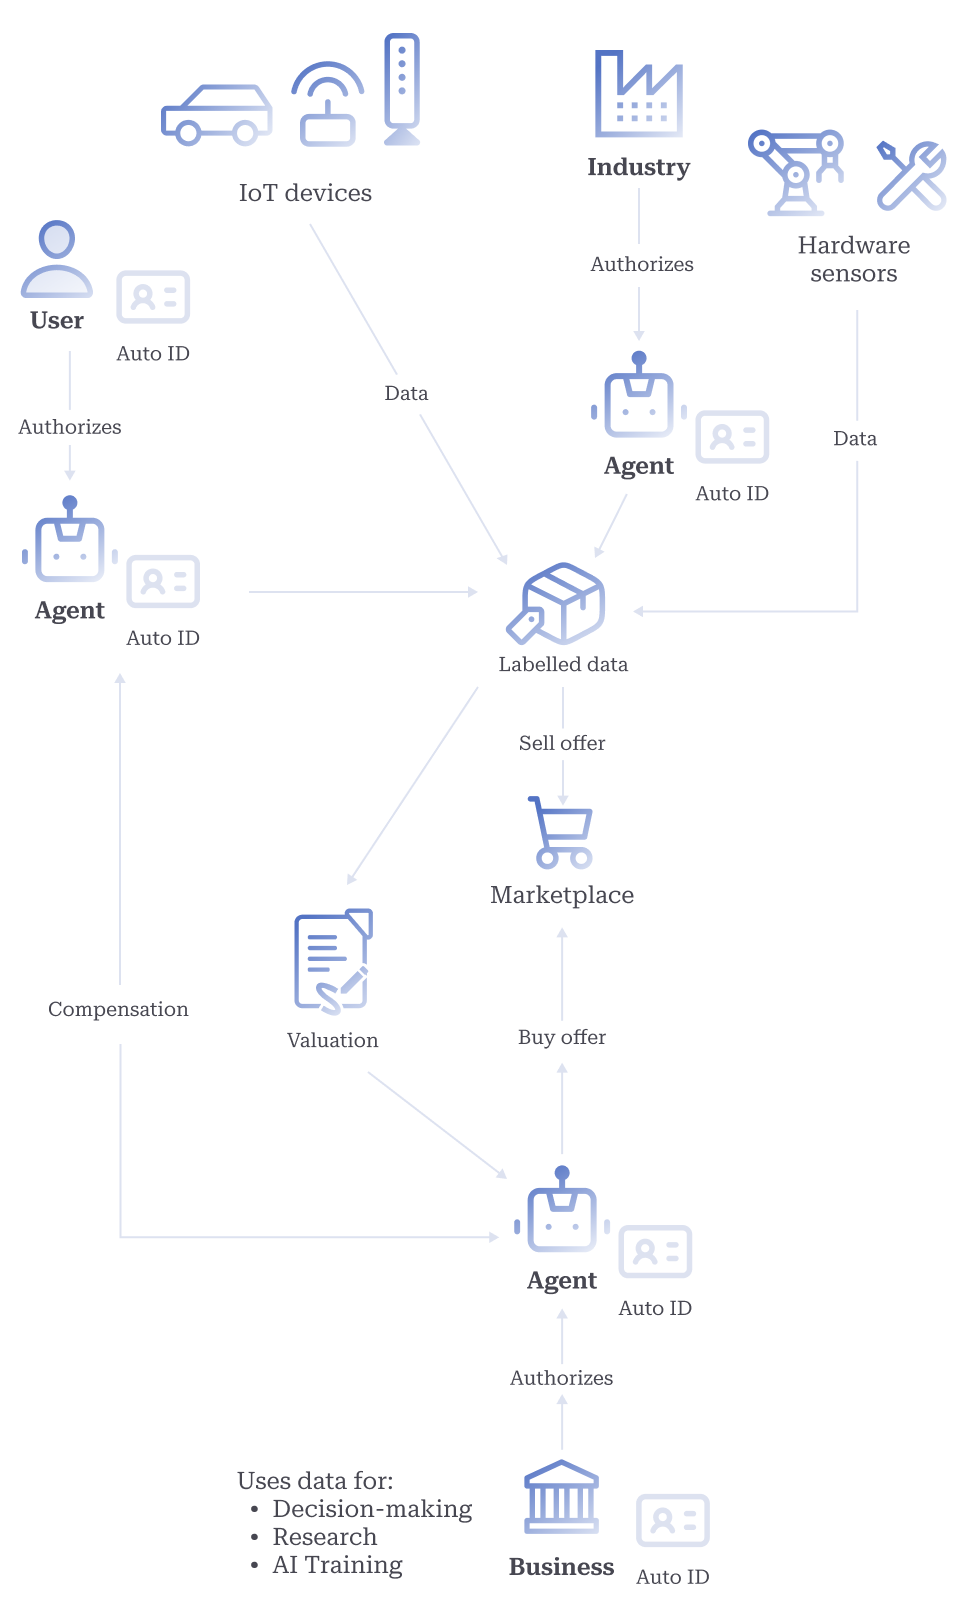
\includegraphics[width=1\linewidth]{data_comp.png}
\caption{Data Contribution and Compensation}
\label{fig:datacomp}
\end{figure}

The Auto ID framework can be leveraged to enable users to participate in decentralized learning initiatives (such as federated learning and swarm learning) by contributing their data to machine learning models, while maintaining privacy and control over their personal information. Decentralized learning allows for model training on distributed datasets without the need for centralized data storage, thereby mitigating risks associated with data breaches and unauthorized access. The integration of decentralized learning with blockchain-based identity and compensation mechanisms represents a significant step towards a more equitable and decentralized AI ecosystem. Moreover, it creates a new paradigm for data ownership and monetization, where individuals can directly benefit from the value their data creates in AI systems (see Fig.\,\ref{fig:datacomp}). This approach aligns with the principles of data sovereignty and deAI, and addresses growing concerns about data privacy and the centralization of AI development\cite{lanier2013}\cite{ibarra2018}.

To incentivize high-quality data contribution and ensure fair compensation, the Autonomys Network will implement a data valuation framework inspired by Shapley-value-based methods \cite{shapley}\cite{pandl2023}, which quantifies individual contributions to the decentralized learning process. It considers multiple factors in its valuation algorithm, including data quality, uniqueness, relevance to the specific model being trained, and the impact on model performance improvements. This approach aims to accurately reflect the true value of each user's data contribution, moving beyond simplistic metrics such as data volume.

The valuation process will be complemented by a compensation mechanism that utilizes the Autonomys Network's native token. The implementation of such specialized mechanisms naturally maps onto Autonomys' domain layer of decoupled execution environments, allowing for independent development and upgradability without burdening the core protocol. This domain will automatically remunerate users whenever their data is accessed or utilized in model training or inference. Given the large number of individual users and data points the system will have to process during every training and inference request, and the number of payouts this will entail, we will employ several optimizations. These include accruing compensation in a smart contract and letting users initiate claims for payouts. All the accrual and claim records on the domain will be anchored and archived within the global history of the chain, ensuring transparency and immutability in recording data usage and corresponding compensation.

The system may also implement a dynamic pricing model that adjusts compensation based on market demand for specific types of data, creating a more efficient data marketplace. As an additional benefit, this approach could potentially lead to more diverse and representative datasets, addressing issues of bias in AI systems that often arise from limited or homogeneous training data.

\subsection{Agent Infrastructure and Multi-Agent Systems}

AI models capable of autonomously interacting with their environment (agents) operating in a distributed environment can collaborate with each other on complex tasks to achieve shared goals as part of multi-agent systems (MAS). The emergent AI agent technology ecosystem, exemplified by projects such as BabyAGI\cite{babyagi}, AutoGPT\cite{autogpt}, and GPT-Engineer\cite{gpteng}, has demonstrated the immense potential of autonomous AI systems. These projects showcase the ability of AI agents to perform complex tasks, engage in goal-oriented behavior, and even recursively improve their own capabilities. At their core, they are based on simple, yet powerful techniques—chains of prompts and responses that decompose large tasks into independent sub-tasks that execute autonomously in a multi-step process before self-validating the output. Frameworks like LangChain\cite{langchain} have extended these agentic capabilities by providing API calls which allow local agents to interact with the ``outside'' world. Chainlink Functions\cite{chainlink} have made web2 APIs composable with blockchain rails and web3 smart contracts. The success of these initiatives has ignited widespread interest in agentics, pointing to a future where AI agents play an increasingly important role in various applications. If each individual and business entity is to have multiple agents acting on their behalf, it is imperative we build the infrastructure to support an economy of billions of these agents. 

Infrastructure for agent deployment differs in their hosting structure and location and in their method of interaction with external service providers and other agents. On the hosting layer, agents can be categorized into specialized agents—that can run exclusively on edge devices using smaller models—and generalized agents—that require high-density GPUs and large amounts of RAM. Generalized agents utilize large frontier models for task decomposition, prioritization and result validation, allowing them more advanced reasoning levels compared with specialized agents, which use smaller, task-specific models. However, specialized agents offer advantages in terms of lower latency, reduced power consumption, and improved privacy due to their ability to operate locally on edge devices. It is thus prudent to assume that there will be a significant heterogeneity of model sizes, hardware requirements and capabilities in use. The Autonomys Network is interoperable with these various platforms owing to its common composable interface and network between domains. Agents that require hardware beyond the self-hosting capabilities of a single user or organization can be programmed to run continuously or on-demand via specialized Autonomys compute-sharing domains. On-chain agents (Autonomys agents) that are in constant high demand may benefit from being deployed on their own domain with specific hardware requirements for operators of that domain.

In addition, agents need digital storage integration for their memory and knowledge base. The Autonomys Network's decentralized storage layer is able to provide this data availability. The most effective agentic decision-making is achieved when agents have access to data outside of their training set, such as information about events that occurred after the training was complete, specialized domain knowledge, or the personal data of the user. Financial trading agents, for example, greatly benefit from access to real-time news from around the world, as do many other applications. The process of factual data retrieval from external sources to enhance the reliability of generative AI outputs is known as retrieval-augmented generation (RAG). Autonomys agents can perform RAG by tapping into the sovereign data economy described in \hyperref[sec:datacomp]{Data Contribution and Compensation} to access data (stored in archival storage) being offered in the marketplace, and compensating the creators for its use (in our native token).

On the higher levels of the stack, Autonomys agents perform tasks on their users' behalf in accordance with user intents. This entails users delegating authority to them to carry out certain permitted activities, including managing user authentication and authorization while interacting with external services, and
accessing their user's financial resources and means of transferring them to pay for goods and services. Every Autonomys agent interacting with the network obtains an identity at deployment, registered through Auto ID, providing verifiable and tamper-resistant agent identities. These IDs may be issued by individuals or organizations with metadata about the agent's purpose and capabilities. Humans, organizations and agents on Autonomys can define hyper-specific permissions for agentic interaction with Auto ID, enhancing security and privacy. Possession of an Auto ID by an agent permits it access to the economic system of the network, allowing it to manage a balance, spend funds and receive payments. All identity claims, authorization events, and agent interactions are provable on-chain, providing a transparent and immutable audit log facilitating accountability and post-hoc analysis. As a unified system for all entities on-chain, Auto ID simplifies the invocation of registered agents for both users and other agents. This agent invocation mechanism is augmented with a distributed reputation system for optimized reliability and performance.

Agent-to-agent communication requires a common interface to facilitate seamless interaction and collaboration on complex tasks, such as organizing a conference, illustrated on Fig.\,\ref{fig:agentscoor}. Autonomys' unified identity framework unlocks composability for agents and cooperation for effective task execution through the advent of multi-agent systems. Each agent can expose endpoints within a shared interface that allow other entities to discover the list of services it provides and actions it is authorized to perform.

\begin{figure}
    \centering
    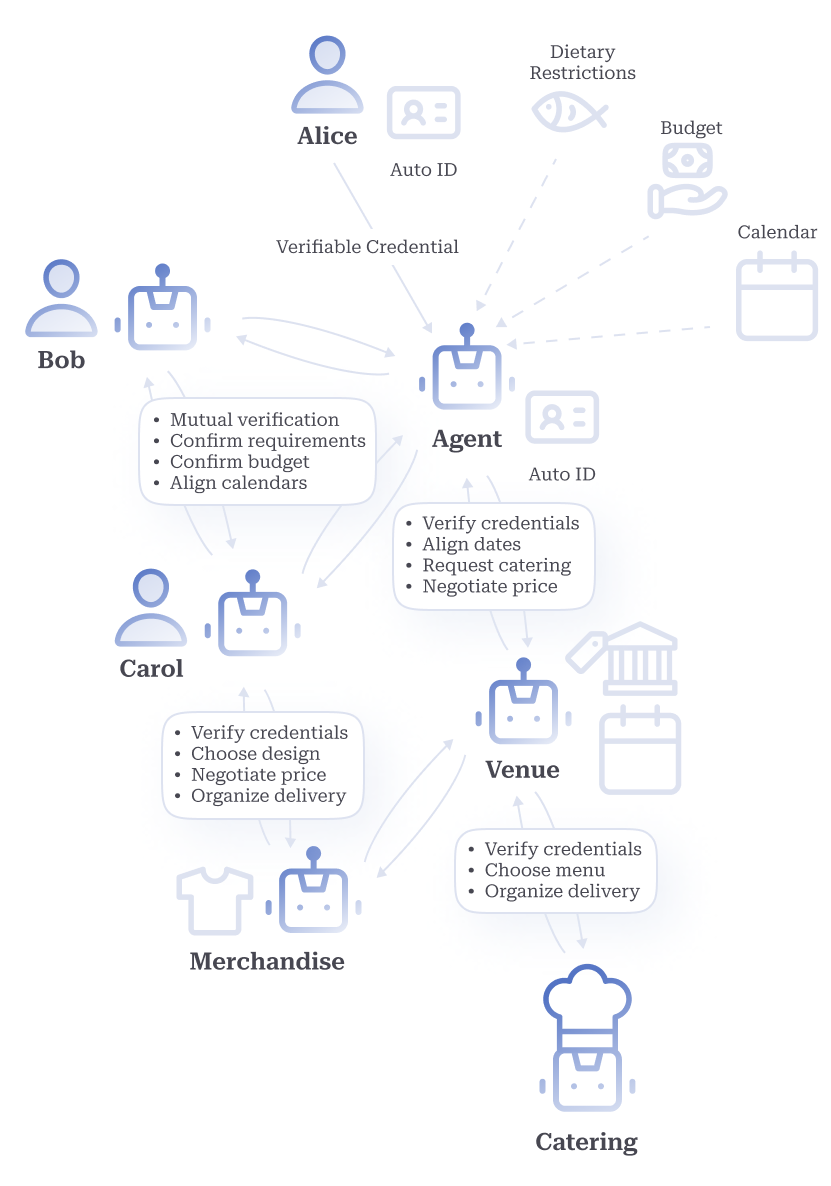
\includegraphics[width=1\linewidth]{multi-agent-system.png}
    \caption{Example of a MAS for coordinating the organization of a conference with a catering service and a merchandise stand:
    \textbf{1)} Alice intends to book a venue for a conference. She authorizes her personal agent to manage her calendar and represent her in specific interactions by signing verifiable credentials (VCs), allowing it to share information with other agents.
\textbf{2)} Alice's agent contacts those of her colleagues, Bob and Carol. Each agent exchanges VCs to verify that they are authorized representatives of their users.
\textbf{3)} Each agent exchanges their user's calendar availability to align their schedules, and confirms the requirements, budget and technical setup for the conference, the merchandise to be distributed and each person's dietary restrictions.
\textbf{4)} Alice's agent initiates a dialogue with the conference venue's customer service agent. Both agents exchange their VCs to ensure they are authorized to make bookings and share sensitive information.
\textbf{5)} The venue's agent verifies availability and confirms the preferred time for the conference. Alice's agent communicates their dietary restrictions to ensure the venue's catering can accommodate them. They discuss the technical setup and space needed for merchandise distribution before negotiating a price.
\textbf{6)} The venue’s agent coordinates with the catering service agent to ensure all dietary restrictions are met.
\textbf{7)} The agents of the merchandise suppliers are contacted to confirm the price, design, delivery and setup of the conference materials and products.
\textbf{8)} All agents use their edit-permission VCs to update their users' respective calendars with the relevant information. The venue’s booking system is updated with the reservation and all specified requirements.}
\label{fig:agentscoor}
\end{figure}

\subsection{Agent Identities}
\label{sec:agentids}
Autonomous agents will operate independently and on behalf of human entities. This paradigm shift necessitates robust mechanisms for accountability. Public key infrastructure (PKI) presents a natural solution, as it is built fundamentally on chains of trust, which establish a verifiable and transparent lineage of trust relationships, ensuring each entity in the chain can be held accountable for their actions, and any breaches can be easily traced. We propose the development of an enhanced PKI system, augmented with additional identity mechanisms, to facilitate the transition to a secure era of human-agent collaboration.

Our proposed Autonomys PKI derives the Auto IDs of any Autonomys agents users build from the Auto IDs of the individual(s) and/or organization(s) that built them. The system provides a secure and transparent mechanism for authorizing the actions of agents within the Autonomys ecosystem via the granting and revoking of granular permissions. This ensures that these AI systems operate within the bounds of their predetermined roles. Permissioned delegation of authority is crucial in a world where digital employees and personal assistant agents make important decisions and perform vital tasks for both organizations and individuals.

Key features of agent Auto IDs include:
\begin{itemize}
    \item \textit{Traceability}: Blockchain tech enables the tracking of agent actions and decisions, supporting auditability and safety in AI development, deployment and alignment.
    \item \textit{Delegation}: Users can securely delegate authority to AI agents, defining their roles and permissions.
    \item \textit{Accountability}: The system maintains a clear chain of responsibility from the agent back to its human or organizational creator.
\end{itemize}

In summary, by enabling users to delegate authority to AI agents; trace the lineage and behavior of agentic systems for safety and regulatory compliance; maintain accountability in digital interactions; and authenticate AI-generated content, Auto ID facilitates much more secure and equitable interaction between humans and AI, establishing a foundation of trust crucial for the autonomous machine economy.

\subsection{Open Collective Intelligence and the Global DAO Mesh}

Recent developments in decentralized autonomous organization (DAO) technology have showcased the numerous avenues of potential they provide for the future of collaborative decision-making and resource allocation\cite{dao} in this new economy. Building upon these foundations, we propose a novel framework that leverages the power of collective intelligence through a network of Auto DAOs interconnected in a Global DAO Mesh.

Collective intelligence—a form of intelligence emerging from collaboration between many individuals—is already being harnessed for effective decision-making and governance by DAOs. Auto DAOs—smaller, specialized DAOs, composed of both human and AI members, deployed on the Autonomys Network—will demonstrate the efficacy of their collective intelligence by managing decentralized projects. Examples include web3 initiatives, investment funds, and research and development for open-source software. When these Auto DAOs are integrated into a larger, interconnected network—the Global DAO Mesh—a more effective and efficient system of collective intelligence emerges.

Autonomys envisions the Global DAO Mesh serving as the decentralized framework for open collective intelligence (OCI)—a more humanistic, albeit AI-augmented, alternative to artificial general intelligence (AGI). OCI operates on the principle of distributed problem-solving, where large, complex challenges are decomposed into smaller, more manageable tasks. These subtasks are then allocated to different Auto DAOs based on their specialized knowledge domains and vested interests in the issue at hand. The process of collective problem-solving via OCI within the Global DAO Mesh can be described as follows:
\begin{enumerate}
    \item \textit{Problem Decomposition}: Complex issues are broken down into independent components.
    \item \textit{Task Allocation}: Subtasks are distributed to relevant Auto DAOs within the mesh.
    \item \textit{Parallel Processing}: The human and AI members of each Auto DAO collaboratively address its assigned component.
    \item \textit{Solution Aggregation}: The Global DAO Mesh aggregates the solutions from individual Auto DAOs (potentially via a round of consensus with a weighted function representing the relative expertise of each DAO).
    \item \textit{Recombination and Synthesis}: The aggregated solutions are recombined to form a cohesive resolution to the original, complex problem.
\end{enumerate}

Inspired by mixture of experts networks (MoE) \cite{moe}, all steps in the process can be mediated via an agentic AI system that understands the necessary context on existing DAOs, their public members' expertise, and the prior participation records of both. This methodology creates a networked intelligence that is both decentralized and scalable, capable of addressing challenges of a magnitude not feasible for individual human or DAO entities. Drawing parallels with the Allora Network\cite{allora}, our proposed system similarly leverages decentralized machine intelligence. However, while Allora focuses on a self-improving AI network, the Global DAO Mesh's OCI emphasizes the synergy between human and AI intelligence within a decentralized governance structure. Autonomys' Global DAO Mesh thus represents a significant advancement in collective problem-solving capabilities. The Global DAO Mesh distinguishes itself via several key advantages:
\begin{itemize}
    \item \textit{Hybrid Intelligence}: Combines the strengths of both human intuition and AI computational power.
    \item \textit{Specialization}: Leverages the unique expertise of different Auto DAOs for optimal problem-solving.
    \item \textit{Decentralization}: Ensures no single point of failure and promotes a truly distributed decision-making process.
    \item \textit{Scalability}: Allows for the tackling of increasingly complex problems by distributing the workload across multiple Auto DAOs.
\end{itemize}

Important research directions to ensure an ethically aligned global decision-making system include optimizing task allocation algorithms to ensure fair representation, developing robust consensus mechanisms for solution aggregation, and exploring the potential for emergent behaviors within the Global DAO Mesh.

%\subsection{Governance and AI Alignment}
%TODO

\subsection{Verifiable AI3.0 Infrastructure as a Public Good}

The provision of a public good infrastructure for accessible, verifiable AI is of paramount importance in our rapidly evolving technological landscape. As highlighted by Korinek and Stiglitz (2019), the advancement of AI technologies has significant implications for income distribution and employment~\cite{korinek2019}. Equal access to AI is crucial if we are to maintain economic relevance and reduce the risk of AI-driven inequality. Democratizing AI entails ensuring that the benefits of these technological advancements are more equitably distributed across society. In pursuit of this goal, Autonomys is committed to establishing infrastructure that offers equal access to verifiable AI agents, tooling and resources as a public good.

A key component of this digital public infrastructure is Autonomys' dedicated directory for the decentralized storage, indexing and distribution of open-source AI data within our extensive, immutable, permanent DSN. The primary objective of our decentralized open-source AI directory is to securely store and make freely available a wide range of valuable AI resources, including:
\begin{itemize}
    \item Open-source AI models
    \item Publicly available training datasets
    \item Fine-tuning datasets
\end{itemize}

At the same time as providing a robust, permissionless, decentralized solution for building and deploying AI models and agents, the Autonomys Network preserves these critical AI assets, ensuring they remain accessible and protected against potential censorship or removal in perpetuity.

\section{The Subspace Protocol}
\label{sec:subspace}
At its core, the Autonomys Network implements Subspace~\cite{subspacev1}, a novel storage-based consensus protocol that separates transaction ordering from execution. The Subspace Protocol was designed from the ground up to enable an open and inclusive Internet by:
\begin{itemize}
    \item Providing an energy-efficient and eco-friendly alternative to proof-of-work (PoW), while still allowing for mass participation by ordinary users.
    \item Creating an incentive-compatible permissionless network that encourages and maintains decentralization over the long term.
    \item Scaling network storage and compute capacity proportional to the number of node operators, without sacrificing decentralization or security.
    \item Connecting and enabling interoperability between existing networks.
\end{itemize}

Achieving this vision required an alternative to both resource-intensive PoW mining and permissioned proof-of-stake (PoS)—a cryptographic proof system based on an underlying resource that is already massively distributed and which does not lend itself to special-purpose hardware. Enter \textit{proof-of-capacity}\footnote{We use proof-of-capacity as an umbrella term encompassing proof-of-space, proof-of-storage, proof-of-replication, proof-of-space-time, proof-of-retrievability, and other storage-based protocols.} (PoC), which replaces compute-intensive mining with storage-intensive farming, under the maxim of one-disk-one-vote. Disk-based consensus is an obvious solution as storage hardware consumes negligible electricity, exists in abundance across end-user devices, and has long been commoditized.

Subspace uses a longest-chain PoC consensus mechanism based on solid-state drive (SSD) storage. Adhering to Nakamoto’s vision, the blockchain is permissionless but secure, with respect to safety and liveness, as long as honest farmers collectively dedicate more storage than any cooperating group of attacker nodes. In essence, Subspace follows the Ethereum model of a fully programmable, account-based blockchain, which periodically commits to the state of all accounts within the block header.

\begin{figure*}
    \centering
    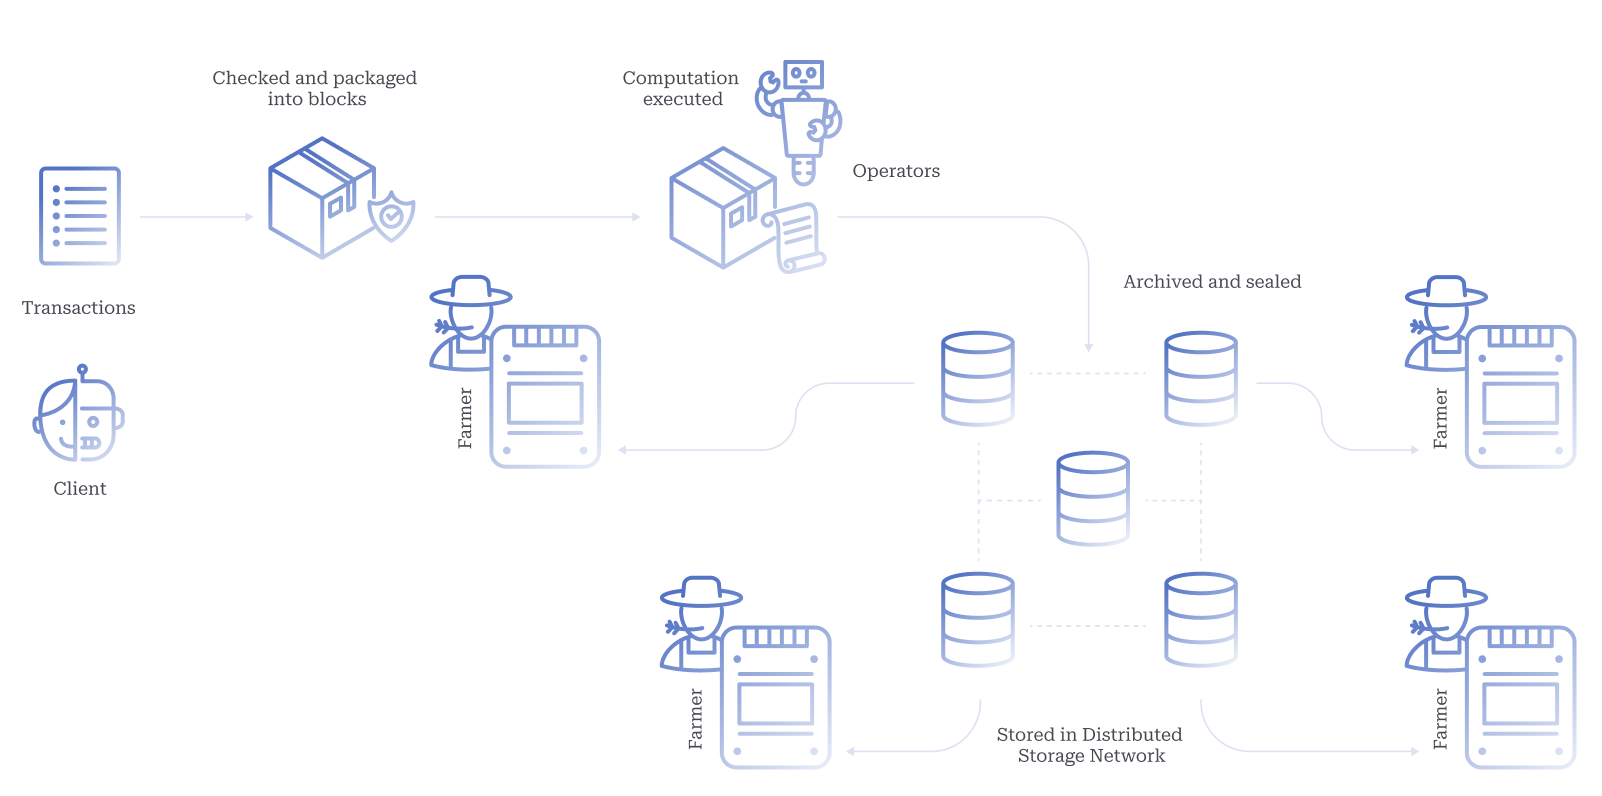
\includegraphics[width=0.75\linewidth]{data-flow.png}
\caption{Blockchain Data Flow}
\label{fig:dataflow}
\end{figure*}

Contrary to many existing PoC protocol designs, Subspace addresses a critical mechanism design challenge—the farmer's dilemma—which poses a significant threat to the decentralization and security of PoC blockchains~\cite{subspacev1}. Rational farmers are incentivized to allocate all their available storage towards consensus, neglecting the maintenance of chain state and history~\cite{lerner2015}. In the farmer's dilemma, this behavior leads to farmers effectively becoming light clients, degrading network security and decentralization. The trend ultimately risks consolidation into large farming pools, centralizing control around pool operators, and reducing the network's resilience against malicious actors. The farmer's dilemma also exacerbates the verifier's dilemma\cite{luu2015} by raising the opportunity cost of verification. If full nodes do not store the chain history, new nodes must instead rely on altruistic archival nodes or third-party data stores for initial synchronization, resulting in a more centralized network.

Subspace circumvents the farmer’s dilemma without sacrificing network security or decentralization as follows (illustrated in Fig.\,\ref{fig:dataflow}):
\begin{itemize}
    \item \textit{To prevent farmers from discarding chain history}: we construct a novel PoC consensus protocol, based on proofs of storage of the blockchain's history (Proof-of-Archival-Storage), where each farmer stores as many provably unique partial replicas of the chain history as their disk space allows.
    \item \textit{To ensure consensus retains the fairness of one-disk-one-vote}: we make the plotting process more computationally intensive than Hellman's time-memory tradeoff\cite{beyond_hellman}, meaning that augmenting or replacing storage with computation is economically irrational for farmers.
    \item \textit{To ensure chain history remains available}: farmers form a decentralized storage network, which allows chain history to remain fully recoverable, load-balanced, and efficiently retrievable.
    \item \textit{To relieve farmers of the burden of maintaining the whole state and performing redundant computation}: we apply the classic distributed-systems technique of decoupling consensus and computation. Farmers are then solely responsible for ordering transactions, while a separate class of operator nodes maintains the state and computes the state transitions for each new block.
    \item \textit{To ensure operators (executors) remain accountable for their actions}: we employ a system of staked deposits, verifiable computation, and non-interactive fraud proofs.
\end{itemize}

\subsection{Proof-of-Archival-Storage}
\label{sec:poas}
To participate in a Proof-of-Archival-Storage (PoAS), farmers first create and store provably unique partial replicas of the chain history, before responding to random, publicly verifiable storage audits, which allow them to forge new blocks. This stands in contrast to the PoC protocols proposed by Spacemint~\cite{spacemint}, Chia~\cite{chia}, and SpaceMesh~\cite{spacemesh}, in which nodes store randomly generated data, rather than useful files. PoAS is inspired by Sergio Lerner's Proof-of-Unique-Blockchain-Storage~\cite{lerner2015} mechanism, but is utilized directly for consensus.

Subspace's PoAS protocol was built to provide a superior user experience (UX) to existing PoC protocols, while maintaining the highest level of consensus security. Its most relevant UX and performance metrics are:
\begin{itemize}
    \item \textit{Setup time}: hours–days (depending on allocated disk space)
    \item \textit{Proof-generation time}: $<$ 1 second
    \item \textit{Proof size}: $<$ 1 KB
    \item \textit{Verification time}: 0.001–0.01 seconds
\end{itemize}
The latest iteration of the Subspace Protocol\cite{subspacev2} uniquely combines KZG polynomial commitment \cite{KZG_paper}, erasure coding \cite{erasure}, and function inverting~\cite{beyond_hellman} to address outstanding design challenges, significantly improving upon previous versions of the protocol\cite{subspacev1}. Below is an overview of the resulting consensus mechanism (see \cite{subspacev2} for a more detailed description).

To create partial replicas of chain history for the farmers to store, we divide the full blockchain history $F$ into $n$ pieces $\{ d_0, d_1, \ldots, d_{n-1}\}$, each of equal size,\footnote{In general, $F$ grows over time. Here, we only consider the case that $F$ is fixed and defer the general case to our protocol specification found at https://github.com/subspace/protocol-specs.} in an \textit{archiving} construction inspired by\cite{semiavidpr} and illustrated in Fig.\,\ref{fig:archiving}. 
\begin{figure}
    \centering
    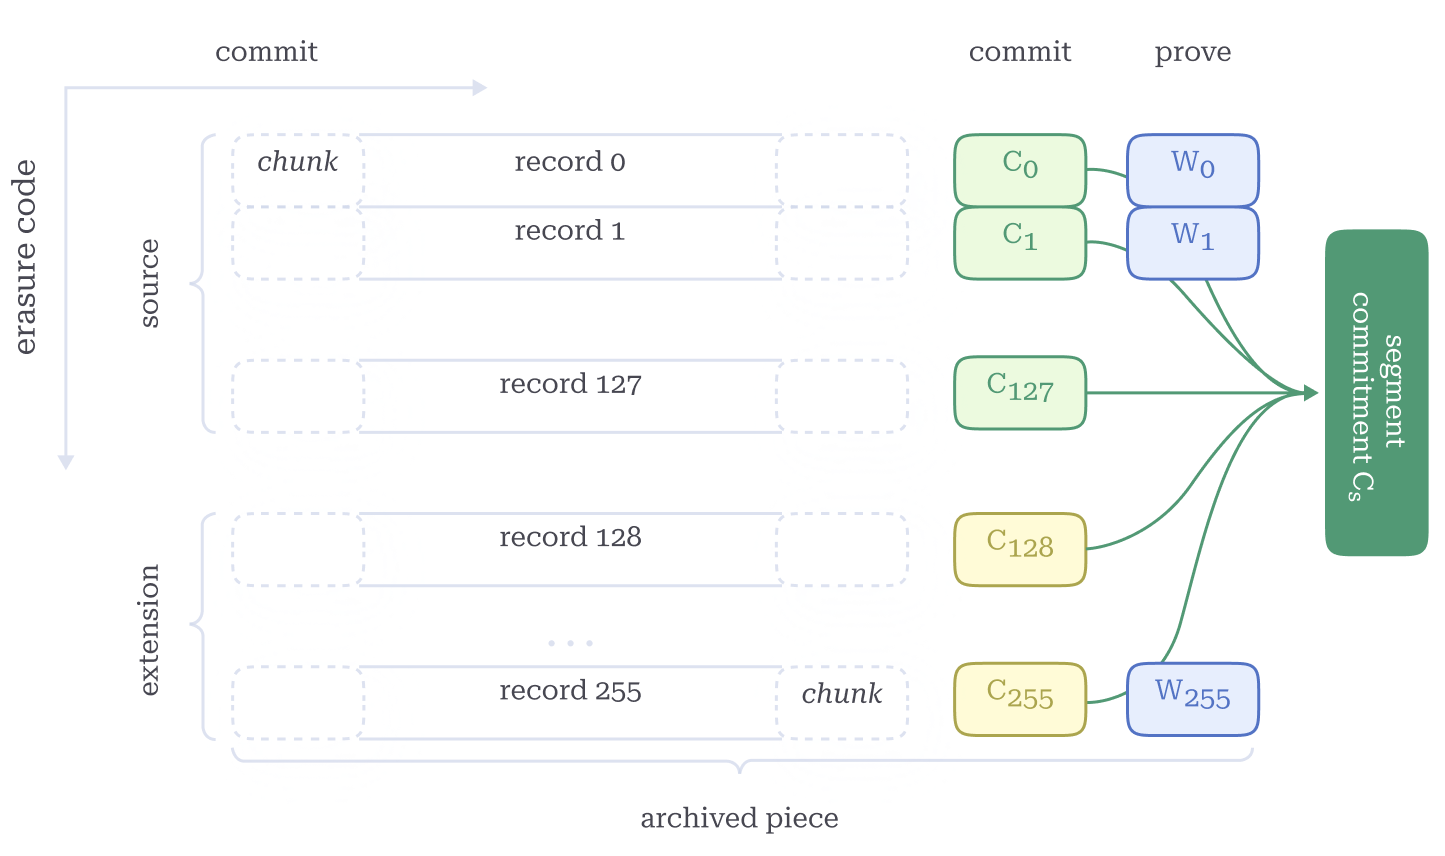
\includegraphics[width=1\linewidth]{archived-segment.png}
\caption{Archived segment}
\label{fig:archiving}
\end{figure}
Without loss of generality, we view each piece as a row vector of length $\ell$ over $\Fp$ (i.e., $d_i \in \Fp^\ell$)\footnote{$\Fp$ because we will apply KZG polynomial commitment later, therefore a prime $p$ has to be compatible with a KZG scheme and sufficiently large}.
Then, $F$ can be viewed as a matrix of size $n \times \ell$ over $\Fp$.
Alternatively, each piece $d_i$ can be viewed as a polynomial $f_i(x)$ over $\Fp$ of degree at most $\ell - 1$. 
This allows us to view $F$ as a collection of $n$ polynomials $\{ f_i(x) \}_{i = 0}^{n-1}$.

Let $A_i$ be the KZG commitment of $f_i(x)$ for $i \in \{0, 1, \ldots, n-1\}$, known as piece commitment, and $T$ is the KZG commitment of $(H(A_0), \ldots, H(A_{n-1}))$ where $H$ is a cryptographic hash function. $T$ is public information.
Let $\pi_i$ be the KZG proof for $H(A_i)$. With $\pi_i$, anyone in the system can verify whether $A_i$ is consistent with the public information $T$ about the history $F$. This process is described in greater detail in \cite{subspacev2}.

In the practical implementation of the protocol in the Autonomys Network, we first divide the history $F$ into segments, where each segment contains the same number of pieces. In this way, archiving is continuous (instead of a one-time process) where the archived history $F$ is periodically updated with new segments of pieces and their respective segment commitments $T_i$ are appended to the tail end of $F$ in ascending order.

To participate in the network, each farmer generates a key pair $(\sk, \pk)$ and derives their farmer $\id$ (e.g., $\id = H(\pk)$)\footnote{This farmer ID also serves as the peer ID of their node on the networking layer.}.
With a given $\id$, the farmer selects $m$ polynomials $\{g_i^{\id}(x) \}_{i = 0}^{m - 1}$ in a verifiable and pseudorandom manner, and retrieves their KZG commitments $\{\cmt\left(g_i^{\id}(x) \right \}_{i = 0}^{m - 1}$ together with the proofs with respect to $T$. The farmer then creates $\ell$ "storage coins" $\{ F^{\id}(\id + j) \}_{j = 0}^{\ell - 1}$ as described in \cite{subspacev2}, where each storage coin can be viewed as $m$ polynomial evaluations at a given point $\id+j$, i.e:
\[
F^{\id}(\id + j) = \begin{bmatrix} g_0^{\id}(\id + j)\\ g_1^{\id}(\id + j)\\  \vdots \\ g_{m-1}^{\id}(\id + j) \end{bmatrix}.
\]
After that, the farmer generates their masked versions $\{\tilde{g}_i^{\id}(x) \}_{i = 0}^{m - 1}$ by using the hard-to-invert function $\mask_{\seed}(\cdot)$ as described in \cite{subspacev2}.
Finally, the farmer stores $\ell$ masked storage coins as well as some metadata (i.e., $m$ commitments $\{\cmt\left(g_i^{\id}(x) \right \}_{i = 0}^{m - 1}$ together with their proofs).
This process is called \textit{plotting}. Note that the parameter $m$ can differ for different farmers, depending on their pledged storage.

Once a farmer has plotted as much storage space as they wish to pledge to the network, they can participate in the leader election. To elect a leader to propose the next block, a global challenge $\mathcal{C}_t$ is generated at time slot $t$, where a new challenge is produced every second, at which point, each farmer selects one masked storage coin and collects from it $m$ entries for a chance to win the challenge (tickets). If a farmer finds a winning ticket, they have to prove the following
\begin{itemize}
    \item the winning ticket (say, $\tilde{g}_i^{\id}(\id + j)$) is indeed close enough to $\mathcal{C}_t$
    \item the unmasked element ${g}_i^{\id}(\id + j)$ is correct and is a member of history $F$
\end{itemize}
\begin{figure}
    \centering
    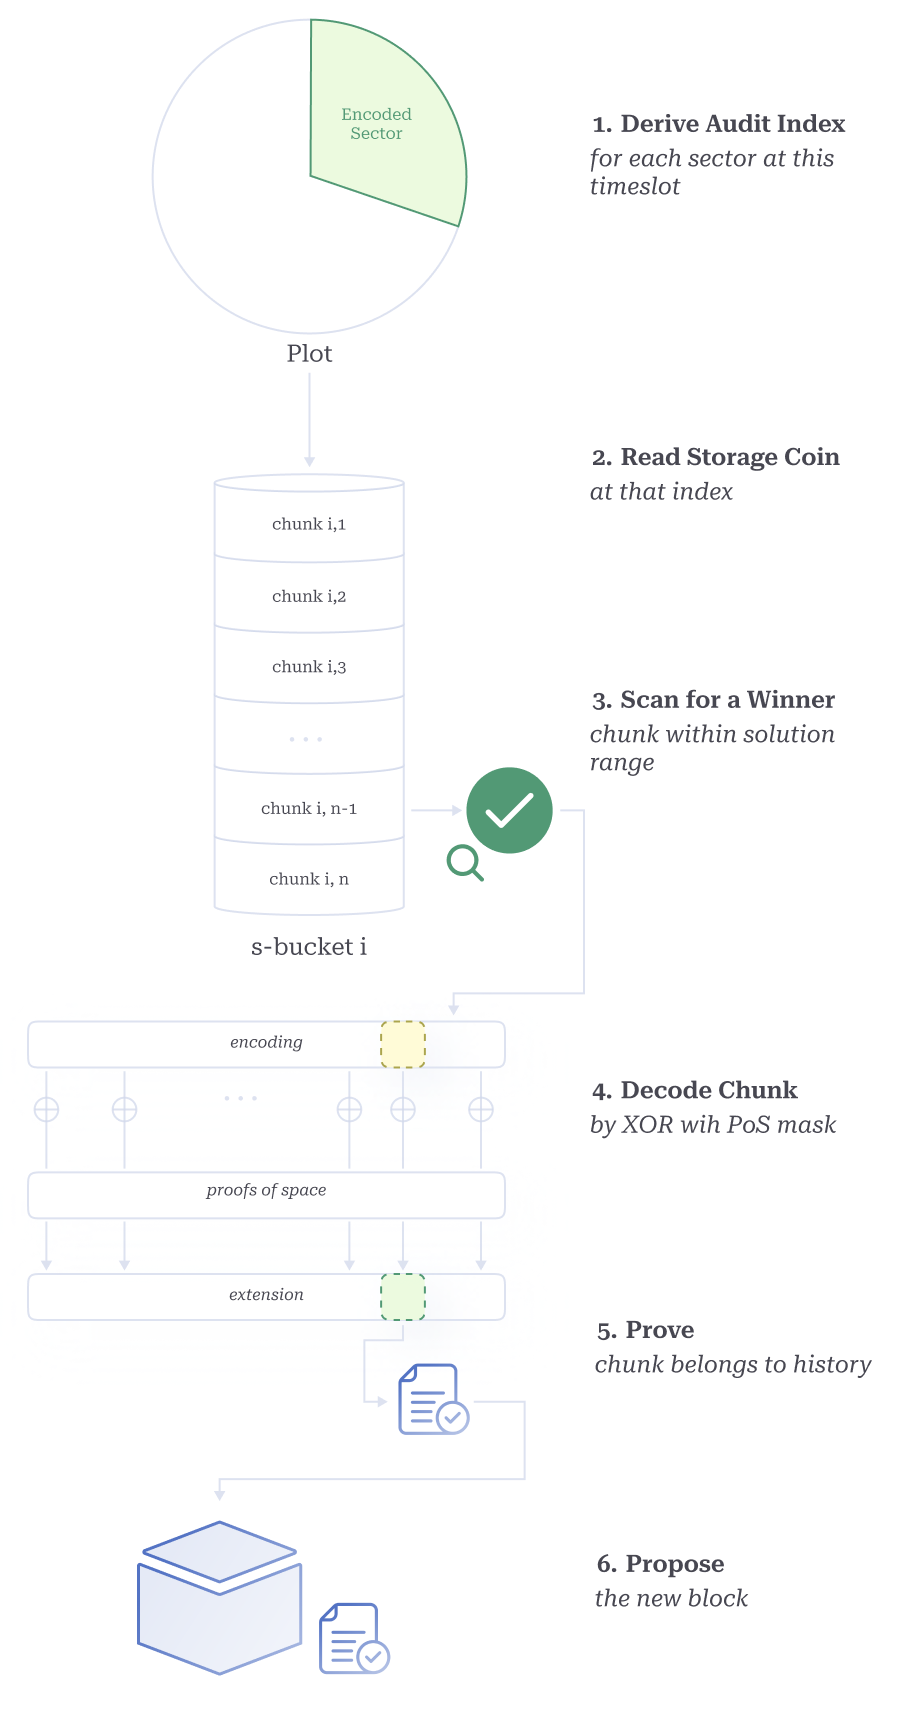
\includegraphics[width=1\linewidth]{farming.png}
\caption{Farming}
\label{fig:farming}
\end{figure}

This process, called \textit{farming}, is illustrated in Fig.\,\ref{fig:farming}. Farming is designed to perform thousands of random reads of small chunks of data per second, making it only feasible on an SSD, further enhancing energy efficiency \cite{ssdvshdd} and decentralization. The above construction provides a leader-election mechanism, which is combined with a longest-chain protocol to produce a consensus algorithm.

\subsection{Proof-of-Time}
\label{sec:pot}
A vulnerability of pure PoS (and by extension PoC) systems lies in their susceptibility to long-range attacks\cite{bagaria2020}. Unlike PoW systems, where block production is physically constrained by computational power, PoS/PoC systems lack this inherent limitation. In PoW, the resource is expended directly to produce a block, and only once, while in PoC the disk space ``resource'' is not tied to a specific block and only provides the eligibility to produce a block, reused over many blocks. Consequently, an adversary with sufficient resources could potentially rewrite a significant portion of the blockchain at any point in the chain's history, compromising its immutability and security. This vulnerability stems from the fact that historical stake distributions can be manipulated without incurring the substantial energy costs associated with PoW systems.

Additionally, PoS/PoC systems often struggle to achieve the dynamic availability and unpredictability inherent in PoW systems\cite{posat}. The challenge lies in creating a system that can adapt to fluctuating participation rates while ensuring that block proposers remain unpredictable, thus preventing targeted attacks or manipulation. These properties are crucial for maintaining robust network operation and security against various attack vectors.

The Autonomys Network addresses these challenges by implementing a separate proof-of-time (PoT) chain that interlinks with the PoAS chain. This design prevents long-range attacks by enforcing a verifiable time constraint between block proposals, analogous to the arrow of time\cite{posat} in PoW systems. PoT guarantees that a certain amount of wall-clock time must elapse between block proposals, preventing an adversary from rewriting history by ``going back in time.'' PoT is constrained physically, similar to PoW, but is not parallelizable (technically, it is proof of \textit{sequential} work), and an attacker cannot immediately generate a successful multi-year retroactive fork even with faster hardware.

The elapsed time guarantee is achieved by iterative evaluation of an inherently sequential delay function. The choice of delay function is crucial to the security and efficiency of the PoT system. After extensive analysis of existing verifiable delay functions (VDFs), we chose to employ repeated AES-128 encryption\footnote{While AES is not technically a VDF, as encryption (proving) and decryption (verification) take the same number of CPU cycles, it can be used as a VDF in practice by parallelizing verification.}. This decision balances security, efficiency and resistance to hardware acceleration. Using the Advanced Encryption Standard (AES) leverages its extensive cryptographic research history and the availability of hardware acceleration in modern CPUs, making it an optimal choice for this application. Based on a joint study with hardware-accelerated cryptography lab Supranational, we do not expect a significant speedup over the best AES implementation, even with an ASIC.

To maintain the PoT chain, the network introduces a new node role called \textit{timekeepers}. These nodes are responsible for evaluating the delay function and disseminating outputs. To provide PoT evaluation, timekeepers require the highest-end CPUs—unavailable to most farmer nodes. Delegating timekeeping to a separate class of nodes ensures decentralization on the consensus level, while maintaining protocol security with minimal honest participation, where the presence of at least one honest timekeeper is sufficient.

To achieve asymmetric verification time for the AES-based delay function, timekeepers publish a set of intermediate checkpoints—currently 8, spaced uniformly—alongside the output (Fig.\,\ref{fig:pot}). Farmers can validate each checkpoint independently and in parallel to reduce overall verification time. Including checkpoints allows other nodes to validate the output $\approx $ 7 times faster and use $\approx$ 4 times less power than evaluation by leveraging instruction-level parallelism.
\begin{figure}
    \centering
    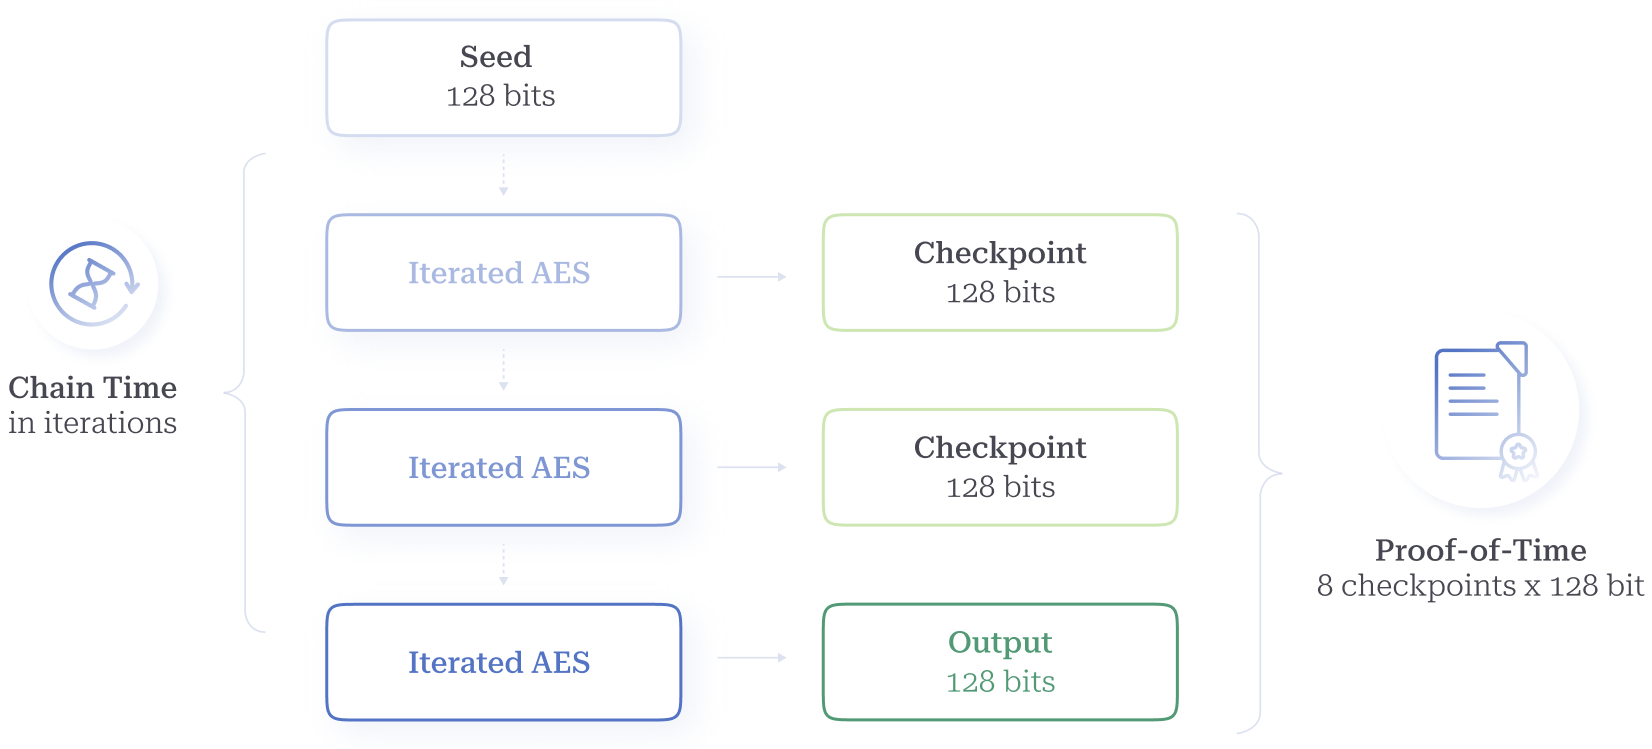
\includegraphics[width=1\linewidth]{proof-of-time.png}
\caption{Proof-of-Time checkpoints}
\label{fig:pot}
\end{figure}

The Subspace consensus protocol utilizes a farming dynamic that mimics the random nature of Bitcoin's mining dynamic, while only expending a small amount of electricity. This is achieved through PoT-based block challenges for the block proposal lottery, based on \cite{posat}. The PoT chain serves as a randomness beacon, providing unpredictable and verifiable inputs for block challenges, thus addressing the issue of long predictability windows often seen in protocols using generic verifiable random functions. This unpredictability is at the same level as that of PoW protocols and is stronger than those using verifiable random functions.

The security of the PoT system is further enhanced by several key mechanisms. Sequentiality is achieved through output chaining between slots, ensuring that each new output depends on the previous one. To compensate for network delays, the system implements a tunable lag parameter, allowing sufficient time for propagation and verification of PoT outputs before block proposals. The Autonomys Network also incorporates measures to mitigate the potential advantage of faster timekeepers, including periodic entropy injection. To prevent manipulation of randomness, the network employs an injection mechanism similar to that used in Ouroboros Praos\cite{ouroborospraos}. This approach prevents attackers from controlling slot challenges by strategically releasing or withholding blocks, further enhancing the unpredictability and security of the system.

\subsection{Distributed Storage}
\label{sec:dsn}
Subspace introduces a distributed storage network (DSN) to ensure consistency of storage over time, given the heterogeneous storage capabilities of farmers. Our DSN design guarantees the following properties:

\begin{itemize}
    \item \textit{Permissionlessness}: The system operates without central coordination, accounting for dynamic farmer availability and non-uniform growth of historical data over time.
    \item \textit{Retrievability}: Both full and single-piece retrieval are facilitated, with requests balanced evenly across all farmers, ensuring that the overhead of serving history remains negligible.
    \item \textit{Verifiability}: Farmers are not required to synchronize or retain the full history, yet the system remains efficiently verifiable.
    \item \textit{Durability}: The probability of any single piece being lost, whether through accidental or malicious means, is minimized.
    \item \textit{Uniformity}: On average, each piece is stored an equal number of times across the network.
\end{itemize}

These features enable the historical data to expand beyond the storage capacity of any individual farmer, while allowing farmers to allocate storage resources according to their individual capabilities.
\begin{figure*}
    \centering
    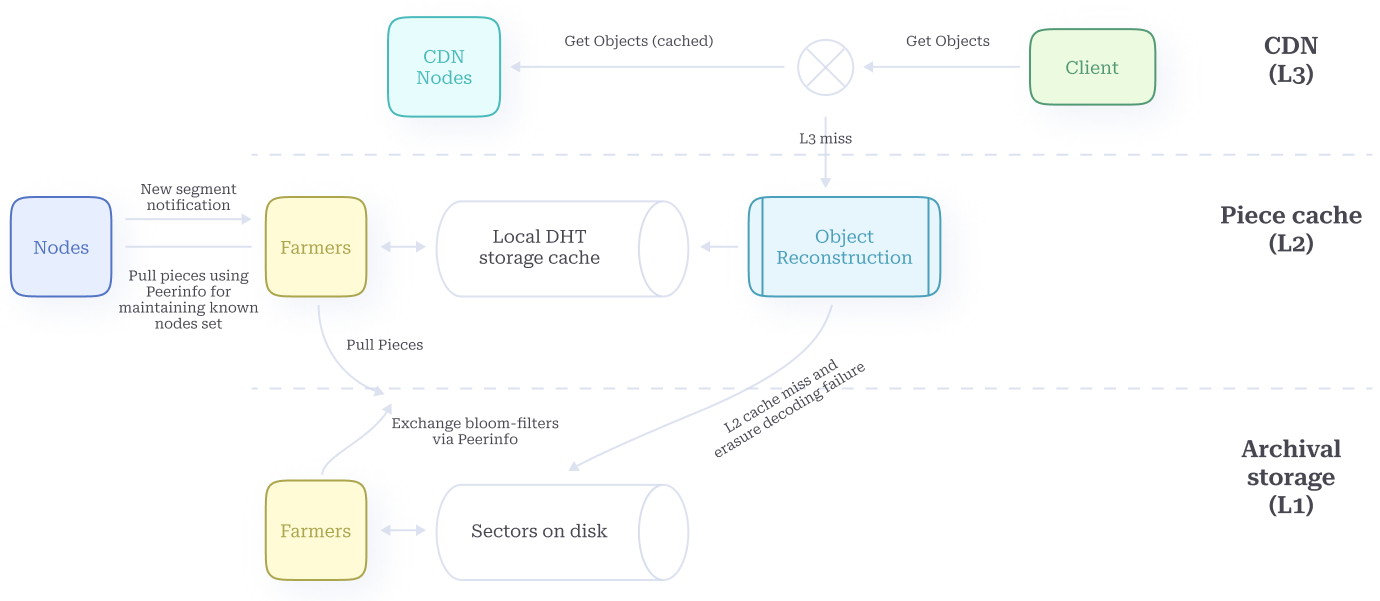
\includegraphics[width=1
\linewidth]{cache-layers.png}
\caption{Distributed Storage Network}
\label{fig:dsn}
\end{figure*}

The Autonomys Network DSN (Fig.\,\ref{fig:dsn}) is comprised of multiple distinct layers that together serve historical data pieces to requesting nodes, with each layer contributing to different aspects of data availability, durability and efficient retrievability. This multi-layered approach was developed to balance security and performance, and interestingly, bears similarities to other recent data availability solutions developed independently from our approach, such as Tiramisu \cite{espresso}.

\paragraph{Content Delivery Network (L3)}

The topmost layer of our DSN is a content delivery network (CDN) designed for optimal performance under optimistic network conditions. The CDN layer (operated by a large permissioned network of nodes) significantly enhances retrieval speed and provides robust performance under normal network conditions. This layer provides web2-like performance for data retrieval:

\begin{itemize}
    \item Farmers upload newly created pieces to the CDN.
    \item Nodes can quickly retrieve pieces from the CDN (similar to downloading from a web2 streaming service).
    \item The CDN serves as an ultra-fast channel for passing messages between nodes, facilitating the rapid collection of data pieces.
\end{itemize}

\paragraph{Pieces Cache Layer (L2)}

The pieces cache layer is designed to facilitate efficient piece retrieval for data reconstruction and farming. Its primary function is to minimize retrieval latency. While retrieval from archival storage necessitates computationally intensive operations by farmers—taking approximately 1 second on consumer hardware—L2 retrieval is near-instantaneous due to the storage of unencoded pieces in the disk cache.

The L2 cache utilizes a distributed hash table (DHT) to store pieces based on the proximity of the piece index hash to the peer ID. Farmers, being the most suitable candidates for L2 storage, allocate a small percentage of their pledged storage for this purpose. The overall storage network replication factor determines the number of farmers storing each piece.

The piece cache layer population process is as follows:

\begin{enumerate}
    \item Nodes generate new segments of pieces during the archiving process.
    \item These new segments are temporarily stored in the node's cache.
    \item Farmers receive the newly archived segment index from the latest block header.
    \item Farmers compute the piece index hashes within the segment and determine which pieces to pull to their L2 based on hash proximity to their peer ID.
    \item Relevant pieces are then pulled to the farmer's local L2 cache.
\end{enumerate}

In the rare case that a specific piece cannot be retrieved to the L2 cache, the farmer will attempt to decode the required piece by requesting its neighboring pieces by index and erasure decoding it from that set. If this fails, the farmer will next attempt L1 retrieval.

\paragraph{Archival Storage Layer (L1)}

The archival storage layer is the fundamental layer responsible for the permanent storage and durability of all chain data. It comprises all storage pledged by farmers for storing masked pieces of chain history, also known as plots. This layer provides the highest level of security against powerful adversaries, albeit at the cost of performance.

Functioning as `cold storage', the archival storage layer ensures the availability of history pieces in the rare event of an L2 cache miss. However, retrieval from archival storage is resource-intensive and time-consuming; thus, it is utilized only when L2 retrieval fails. Typically, the L1 layer of farmers is populated with pieces received from L2.

The archival storage layer population process is as follows:

\begin{enumerate}
    \item The farmer decides how much storage to allocate to the network.
    \item Based on the amount of storage pledged, the farmer pseudorandomly and verifiably selects enough pieces of history to fill that space.
    \item The farmer pulls the selected pieces from the L2 or L1 of other farmers.
    \item The farmer masks the pieces as described in the plotting protocol.
    \item Every time a new segment is archived, the farmer runs a check to see whether they need to replace any pieces.
\end{enumerate}

The last step is necessary to ensure that new history gets replicated uniformly across many farmers in the network, regardless of how long they have been participating in the network or how long ago they initialized their plots. This plot expiration is set up such that the farmer gradually replaces subsets of pieces in the plot as the history of the chain grows. On average, by the time the history has doubled in size, as compared to when the plot was initialized, half of the farmer's plot will have expired and been replotted. By the time the history quadruples, the farmer will have replotted their whole plot once over. The choice of gradual expiration instead of full farm replots ensures maximum uptime of the farmers' archival storage layer for serving pieces to the DSN.

\paragraph{Cache Types}

Separately from the above cache layers, we distinguish the following types of cache:
\begin{itemize}
    \item \textit{Node cache}: Contains newly created pieces from the most recent archived segments. It is limited to a few recent segments and progressively replaces older pieces with new data.
    \item \textit{Farmer cache}: Contains pieces in the L2 cache, automatically populated upon receipt of new archived segment announcements. Pieces are cached according to their proximity to the farmer's peer ID.
    \item \textit{Object cache}: Contains recent and popular user-uploaded objects and their mappings to pieces.
\end{itemize}

To incentivize the farmer network to maintain the desired replication factor for historical data, Subspace implements a novel algorithm that dynamically adjusts the cost of on-chain storage, or \textit{blockspace}, in response to fluctuations in storage supply and demand.

\subsection{Decoupled Execution}
\label{sec:decex}
It is safe to assume that rational farmers will seek to dedicate all their available disk space to consensus and expend as little computation as possible, while remaining on the longest valid chain, meaning they must compute all intermediate state transitions and maintain the state. As the burden of maintaining the state and computing transitions grows larger, both the farmer’s and verifier’s dilemmas present themselves, leading economically rational farmers to sacrifice security for higher rewards at a lower cost, by either becoming light clients or joining a trusted farming pool. To resolve these dilemmas, we implement a method that relieves farmers of this burden, while still allowing them to be certain they are extending the longest valid chain. Critically, this method does not degrade the liveness, fairness, or safety of block production. Our solution follows the classic technique in distributed systems of decoupling consensus and computation.

In this system, farmers are solely responsible for providing subjective and probabilistic consensus over the ordering of transactions. A separate class of executor nodes—operators—computes the objective and deterministic result of that ordering. Operators are selected through a stake-based election, separate from block production, analogous to the block finalization technique proposed by Casper FFG\cite{casper}. They are incentivized by transaction fees shared with farmers, and held accountable through a system of non-interactive fraud proofs\cite{albassam2018} and slashing\cite{buterin2014}.

This approach, while influenced by Flow\cite{flow1, flow2, flow3}, is simpler (using two, not four, classes of nodes), retains compatibility with Nakamoto consensus, and maintains the `honest \textbf{majority} of farmers' and `honest \textbf{minority} of operators' security assumptions. It also draws inspiration from Truebit\cite{truebit}, recognizing that optimistic off-chain computation with fallbacks to on-chain verification could realize a trustless decentralized mining pool. Unlike protocols such as ChainSpace\cite{chainspace} and LazyLedger\cite{lazyledger}, which achieve decoupling by delegating computation to clients, our system retains global state, allowing for cross-contract calls and composability of applications.

Under the decoupled execution (DecEx) framework, farmers only confirm the availability of transactions and provide an ordering, while secondary networks of staked operator nodes execute the transactions and maintain the resulting chain states. DecEx separates the probabilistic process of coming to a consensus over the ordering of transactions from the deterministic process of executing these ordered transactions, as illustrated in Fig.\,\ref{fig:decex}. The decoupling of these roles permits alternative hardware requirements for different node types, allowing us to keep farming lightweight and open to anyone, while also providing a foundation for scaling execution both vertically—based on the hardware capabilities of operators—and horizontally—by partitioning operators into different namespaced execution domains.

While conceptually similar to rollups on Ethereum, such as Optimism, DecEx differs heavily in its protocol implementation. Unlike Ethereum, the Autonomys Network does not have a global smart contract execution environment within the core protocol. Instead, DecEx is enshrined within the semantics of the core protocol itself. Despite being implemented at the protocol level, DecEx is still able to provide rollup protocol designers with a flexible system capable of supporting any state transition integrity framework for verifying the receipt chain, including optimistic fraud proofs and zero-knowledge proofs. DecEx also supports any smart contract execution environment that can be implemented within the Substrate framework, such as the Ethereum Virtual Machine (EVM) or Web-Assembly (WASM).

\begin{figure*}
    \centering
    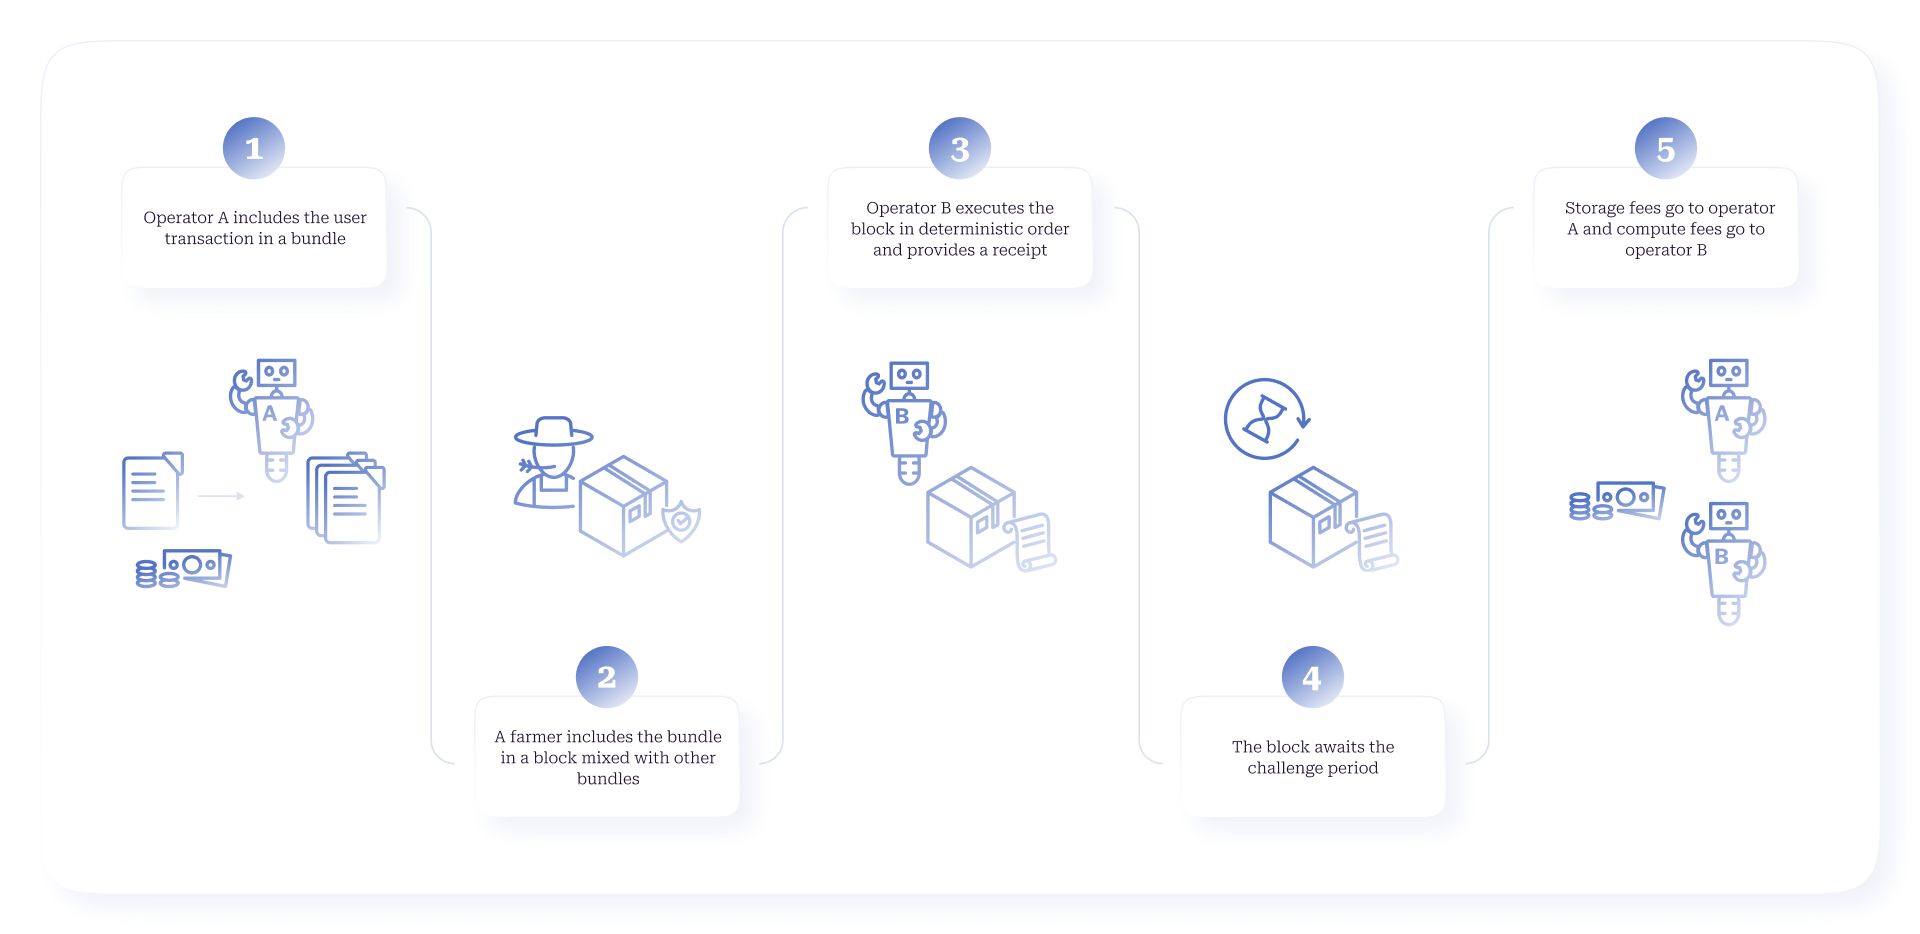
\includegraphics[width=1\linewidth]{domain-flow.png}
\caption{Domain transaction flow from submission to fee distribution}
\label{fig:decex}
\end{figure*}

\paragraph{Domains}

Domains are the logical extension of the basic DecEx framework, taking it from a single, monolithic execution environment to a modular, interoperable network of namespaced execution environments. Each domain is its own programmable layer-2 rollup, or application-specific blockchain (app-chain), that relies on the consensus chain for consensus, decentralized sequencing, data availability, and settlement. However, a smart contract, (super) dApp, or agent can use multiple domains to achieve a complex task, enabled by our unique cross-domain communication.

\paragraph{Farmer Role}

In our DecEx model, users submit execution transactions directly to operators, who pre-validate and batch these transactions into bundles through a (probabilistic) stake-weighted election process. These bundles are then submitted to farmers, who treat them as base-layer transactions. Farmers only verify the proof-of-election and ensure the data is available, before batching bundles into blocks in the usual manner. When a farmer finds a PoAS solution that satisfies the storage audit, they order valid transactions into a new block, committing to the last valid state root proposal they observe. Unlike on Ethereum and most other L1s, farmers do not need to maintain the code, state or account balances for contracts, only the smaller set of balances and nonces for externally owned accounts (EOAs), and minimal information about each domain runtime, staked operators, and execution receipt (ER) chains. The farmer network effectively provides decentralization-as-a-service to the domains.

\paragraph{Decentralized Sequencing}

Once the bundled transactions are included in the consensus block by farmers, domain operators must execute them in a deterministic order based on a verifiably random seed from the consensus chain. This absolves the operators of the responsibility of sequencing user transactions, while also preventing them from harvesting the maximal extractable value (MEV) and causing economic harm to users. Bundled transactions from a domain are opaque to the farmer block proposer as the latter does not have the domain state. Thus, the farmer cannot participate in MEV extraction either. Neither the order in which the operator batches the transactions in the bundle nor the order of bundles in the consensus block influences the final sequencing for execution.

\paragraph{Operator Role}

Operator nodes maintain the full state of their respective domain and execute transactions, returning new proposed state roots. For each new block, a small constant number of operators are chosen through a stake-weighted election. Execution transactions from the block are then ordered deterministically, using a secure cryptographic shuffle based on the unique PoAS produced by the farmer. Operators execute the transactions according to this ordering, and produce a deterministic state commitment in the form of an execution receipt, incrementally committing to intermediate state roots. These state commitments are then included in the next bundle, forming a deterministic receipt chain tracked by all farmers within the consensus chain protocol. The initial, default implementation of DecEx employs an optimistic fraud-proof validation scheme.

\paragraph{Liveness}

To retain liveness in case of network asynchrony or byzantine actors, operator elections are re-run for each new time slot. This allows newly elected operators to include past ERs to catch up. The election threshold dynamically adjusts based on observed operator availability. Each domain may specify the frequency of re-election based on its own needs and demand, without interfering with the liveness of other domains or the consensus chain.

\paragraph{Fairness}

Fairness is preserved through a fair compensation mechanism between farmers and operators. Farmers are compensated for their blockspace at the current price of storage, by rewards, and for their work of including the domain bundles, by the operators. Operators are compensated for the blockspace costs incurred if their ERs are valid, and for their work of bundling and executing user transactions, via transaction fees.

\paragraph{Validity}

Validity is ensured through a system of fraud proofs. Within the challenge period, any honest node which operates on a domain can compile a fraud proof for an invalid state transition performed by another operator on that domain. The fraud proof can be verified by any consensus node without having the whole domain state. If it is valid, the operator who proposed the invalid ER will have their entire deposit confiscated. Any operator who has extended the invalid ER is also slashed as punishment for dishonest or lazy behavior.

\paragraph{Finality}

Transactions on optimistic domains are subject to a challenge period until they are settled on the consensus chain. During the challenge period, nodes can dispute the correctness of state transitions presented by operators. Any node that has an up-to-date state of the domain can submit fraud proofs for this domain and does not need to be a staked operator to do so. Whether the node is acting honestly or not in this particular instance is determined by the validity of the fraud proof. Currently, the challenge period on domains is 14400 blocks, or approximately 1 day. Fast finality is possible for services that run their own honest operator nodes. Since the operator nodes execute all the state transitions, they can be certain about the correctness of the domain state at any given time.

\paragraph{Safety}

Safety is maintained by distinguishing between illegal and invalid transactions. Farmers enforce legality by ensuring transactions have valid signatures and can cover the specified fees. Operators enforce validity by executing transactions deterministically in the order specified by farmers.

\paragraph{Network Dynamics}

Our system is able to account for network delays and stochastic block production. Operators are incentivized to generate fraud proofs locally to release their own ERs as soon as possible, speeding up fraud-proof propagation and strengthening security guarantees. Farmers order by urgency and deduplicate fraud proofs in their mempool to ensure timely inclusion.

\paragraph{Adversarial Scenarios}

The system is designed to handle various adversarial scenarios, including attempts to attack the liveness of execution or confuse farmers about transaction legality. Even in the presence of a dishonest majority of operators, the system remains secure as long as a single honest operator remains connected to an honest farmer within their peer set. Operators are incentivized to reveal fraud to protect their own stake and claim their share of the rewards, while they are punished for extending an invalid ER without first demonstrating fraud.

\paragraph{DecEx Summary}

Our decoupled execution system allows for significant scalability improvements over monolithic execution environments (like Ethereum) by independently scaling transaction throughput and storage capacity. It preserves the security properties of the Nakamoto consensus, even in the presence of a dishonest majority of operators, given an honest majority of farmers on the consensus layer.

Our approach provides a unique solution to the challenges faced by storage-based blockchains, offering a balance between permissionless farming and permissioned staking. Unlike hybrid PoC/PoS consensus mechanisms employed by other storage-based blockchains, Autonomys' system clearly distinguishes between a permissionless farming mechanism for block production and a permissioned staking mechanism for block finalization.

By simultaneously addressing the farmer's dilemma, verifier's dilemma, and blockchain bloat issues, the Autonomys Network presents a comprehensive solution to several critical challenges in the web3 industry, at the same time as making blockchains more energy-efficient, egalitarian and decentralized, and maintaining the security and functionality necessary for complex smart contract and application development.

\section{Scalability}
\label{sec:scalability}
Blockchain scaling has received extensive attention over the past decade. Numerous scalability protocols have been proposed in the literature, including the likes of Prism \cite{bagaria2019prism} and OmniLedger\cite{omniledger}. Building on this existing research, Autonomys is taking a first-principles approach to scaling the Subspace Protocol. The section below outlines this approach to scalability and its implementation.

\subsection{Constraints to Scaling Blockchain TPS}

For any blockchain system, there are at least three physical scaling constraints:
\begin{itemize}
    \item the \textit{communication} constraint—the upload bandwidth of a single participating node.
    \item the \textit{computation} constraint—the number of transactions a node is capable of executing per second.
    \item the \textit{storage} constraint—the number of transactions stored by each node.
\end{itemize}
The goal of blockchain scaling\footnote{Delay is another important metric for blockchain scaling, but is beyond the scope of this whitepaper.} is to achieve the maximum possible throughput under these physical constraints, measured by TPS (transactions per second).

In a conventional blockchain design, a participating node (often referred to as a full node or a miner) has to download, store and execute all the transactions. This requirement leads to several upper bounds. For instance, the throughput cannot exceed the average upload bandwidth divided by the average size of transactions. Thus, if the average bandwidth is 10 Mbit/s and the average size is 250 bytes, the throughput cannot exceed 5000 TPS under the communication constraint—too small for certain applications. The huge number of transactions generated by the future Internet-of-Agents \cite{ioa}, as well as the mainstreaming of the burgeoning decentralized finance (DeFi), decentralized science (DeSci) and on-chain gaming (GameFi) ecosystems, will significantly expedite the demand for greater scalability. How can we scale the Autonomys Network throughput by 100x to be able to handle 500,000 TPS?

\subsection{Scaling the Autonomys Network}

In order to achieve this goal throughput of 500,000 TPS, we could increase the upload bandwidth to at least 1Gbit/s. However, this would sacrifice decentralization, as nodes with low bandwidth would no longer be able to participate. Instead, having already decoupled the requirement that every node store and execute all transactions, via our DSN and DecEx, we are now decoupling the bandwidth requirement.

Inspired by the similarities between rollup and sharding designs \cite{vitaliklayer22024}, we propose a unique sharding approach based on cryptographic sortition. Our system consists of a beacon chain and multiple data shards. The beacon chain is maintained by all the farmers through the PoAS consensus algorithm. Each data shard is maintained by a subset of farmers selected by cryptographic sortition over time. For instance, a farmer could be elected as a leader for the beacon chain if they have a lottery ticket close enough to $\mathcal{C}_t$ (i.e., the distance between the ticket and $\mathcal{C}_t$ is smaller than a threshold $T_b$); elected as a member for data shard $1$ if the distance is no smaller than the threshold $T_b$, but smaller than $T_b + T_s$; elected as a member for data shard $2$ if the distance is no smaller than $T_b + T_s$, but smaller than $T_b + 2 T_s$; and so on. Generally, a farmer is elected as a member for data shard $i$ if the distance is no smaller than $T_b + (i - 1)T_s$, but smaller than $T_b + iT_s$. A farmer is only assigned to a shard when elected and is a member of at most one shard at any time. This \emph{dynamic} shard membership is recorded on-chain as farmers prove their winning tickets.

When a new domain joins, it is assigned to a data shard. 
A farmer elected as a leader for this shard downloads recent blocks and transaction bundles, then produces a new shard block on the longest available chain. 
This new block is shared with domain operators, the DSN, as well as future leaders.
Its block header is shared with all the farmers through gossiping (to be included in the beacon chain).
This process is a variation of Nakamoto’s longest chain protocol, and the majority of leaders in any shard are honest due to cryptographic sortition, which supports shard safety and liveness with high probability.

To address data withholding attacks, where a malicious shard leader colludes with malicious domain operators, the system allows future shard leaders to detect such attacks. For rare undetected attacks, we propose an on-chain complaint mechanism similar to \cite{tas2023}. This workflow is illustrated for one domain and shard in Fig.\,\ref{fig:scalability}.


\begin{figure}
    \centering
    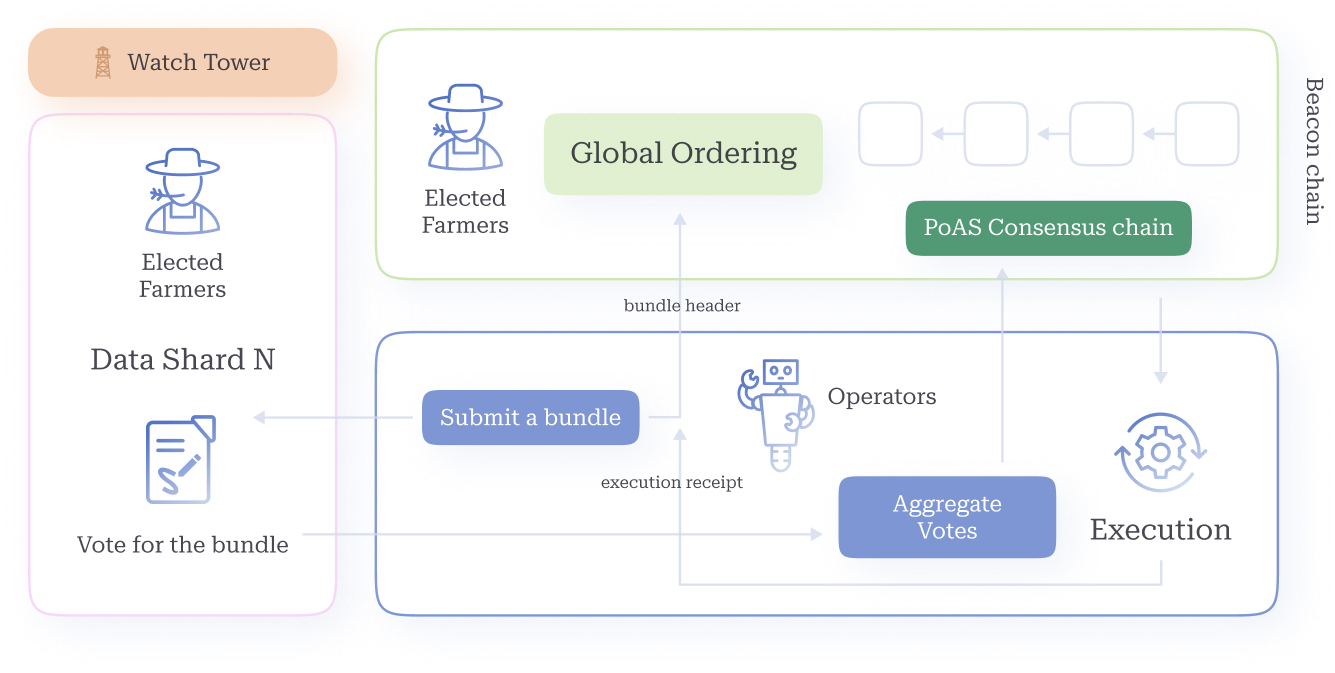
\includegraphics[width=1\linewidth]{shard.jpg}
 \caption{Data flow between domain, shard and beacon chain}
\label{fig:scalability}
\end{figure} 

Next, we present an alternative design using cryptographic sortition and erasure coding. In this setup, explicit shards are unnecessary. When a domain operator creates a transaction bundle, it broadcasts the header to all the farmers (to be included in the beacon chain) and disseminates erasure-coded chunks. Farmers receiving a chunk can vote for the bundle via cryptographic sortition, with voting data recorded on the beacon chain to facilitate consensus on data availability. This is in spirit similar to a very recent scalability design proposed in \cite{rollup2024}.

\section{Conclusion}

The Autonomys Network represents a dual solution to both the:
\begin{itemize}
    \item challenges of security, decentralization, verifiability and scalability facing web3 infrastructure—embodied in the farmer's and verifier's dilemmas, and the blockchain trilemma.
    \item risks and opportunities posed by the emerging AI-augmented world.
\end{itemize}

In implementing our cutting-edge blockchain technologies, we have not only built a robust, decentralized system that addresses the immediate challenges of permanent storage, provenance and compensation for AI training data, but through our verifiable AI3.0 infrastructure and Auto ID, also laid the groundwork for a future where humans and Autonomys agents can interact in a transparent, secure, and trustworthy manner. 

The Autonomys Network stack, composed of the dApp/agent, domain (DecEx), consensus (PoAS), and storage (DSN) layers, forms a comprehensive ecosystem that enables unprecedented scalability, security and flexibility for AI and dApp developers. Our permissionless peer-to-peer network allows for wide participation, while the Subspace Protocol's Proof-of-Archival-Storage consensus mechanism ensures efficient and environmentally friendly operation. The Autonomys Network's modular architecture, with its distributed storage network and decoupled execution domains, offers unparalleled scalability and adaptability. Our design allows for the seamless integration of various state transition frameworks and execution environments, fostering interoperability and innovation across different blockchains. Key innovations Auto ID and Auto Score provide a secure, verifiable identity system for both humans and AI entities that helps address the fundamental challenge of establishing trust in an increasingly AI-integrated world, at the same time as allowing for content authentication, and delegation of permissioned authority.

As well as seeking to drive innovation and growth in the AI and blockchain spaces, we want to empower individuals with self-sovereignty over their digital identities and economic relevance, and ensure the benefits of technological advancement are accessible to all, regardless of their resources or background. We envision the Autonomys Network as the fair, open-source and collaborative foundation layer for AI3.0—an ecosystem for accessible, verifiable and secure dApp and deAI development, deployment and interaction.

\section*{Acknowledgements}
The authors would like to thank Tianyu Shi and Saeid Yazdinejad (University of British Columbia) for their contributions to the scalability roadmap; Barak Shani for his contributions to the Subspace protocol security; Jianming Liu, who coined AI3.0; the Autonomys Labs team, especially Jeremy Frank for contributions to Auto ID, and Chris Sotraidis and Charlie McCombie for their valuable feedback.


\begin{thebibliography}{}

\bibitem{lecun2015} 
LeCun, Y., Bengio, Y., and Hinton, G. \emph{Deep learning} Nature, 521(7553), 436-444, http://dx.doi.org/10.1038/nature14539, 2015.

\bibitem{frey2017} 
Frey, C. B., and Osborne, M. A. \emph{The future of employment: How susceptible are jobs to computerisation?} Technological Forecasting and Social Change, 114, 254-280, https://doi.org/10.1016/j.techfore.2016.08.019, 2017.

\bibitem{brynjolfsson2014} 
Brynjolfsson, E., and McAfee, A. \emph{The second machine age: Work, progress, and prosperity in a time of brilliant technologies} W. W. Norton \& Company, 2014.

\bibitem{zheng2017} 
Zheng, Z., Xie, S., Dai, H., Chen, X., and Wang, H. \emph{An overview of blockchain technology: Architecture, consensus, and future trends} In 2017 IEEE International Congress on Big Data (BigData Congress), 557-564, IEEE, https://doi.org/10.1109/BigDataCongress.2017.85, 2017.

\bibitem{oneil2016} 
O'Neil, C. \emph{Weapons of math destruction: How big data increases inequality and threatens democracy} Crown Publishing Group, 2016.

\bibitem{bostrom2014} 
Bostrom, N. \emph{Superintelligence: Paths, dangers, strategies} Oxford University Press, 2014.

\bibitem{russell2019} 
Russell, S. \emph{Human compatible: Artificial intelligence and the problem of control} Viking, 2019.

\bibitem{miessler}
Miessler, D. \emph{AI's Predictable Path} Unsupervised Learning, https://danielmiessler.com/p/ai-predictable-path-7-components-2024, 2023.

\bibitem{apple}
Apple. \emph{Apple Intelligence} https://www.apple.com/apple-intelligence/, 2024.

\bibitem{altman2021}
Altman, S. \emph{Moore's Law for Everything} https://moores.samaltman.com/, 2021.

\bibitem{subspacev1}
Wagstaff, J. \emph{Subspace: A Solution to the Farmer’s Dilemma} https://cdn.prod.website-files.com/61526a2af87a54e565b0ae92/617759c00edd0e3bd279aa29\_Subspace\_\%20A\%20solution\%20to\%20the\%20farmer\%27s\%20dilemma.pdf, 2021.

\bibitem{subspacev2}
Feng, C., Porechna D., Shani B., and Wagstaff J. \emph{(WIP) Dilithium: A Proof-of-Archival-Storage Consensus Protocol for Subspace}
https://github.com/subspace/consensus-v2-research-paper/blob/main/consensus\_v2.pdf, 2023.

\bibitem{hasan2009} 
Hasan R., Sion R., and Winslett M. \emph{The Case of the Fake Picasso: Preventing History Forgery with Secure Provenance} in Proceedings of the 7th USENIX Conference on File and Storage Technologies (FAST '09), 1-14, USENIX, http://usenix.org/event/fast09/tech/full\_papers/hasan/hasan.pdf, 2009.

\bibitem{westerlund2019} 
Westerlund M. \emph{The Emergence of Deepfake Technology: A Review} Technology Innovation Management Review, 9(11), 39-52, http://doi.org/10.22215/timreview/1282, 2019.

\bibitem{brundage2020} 
Brundage M., Avin S., Wang J., et al. \emph{Toward Trustworthy AI Development: Mechanisms for Supporting Verifiable Claims} arXiv:2004.07213 [cs.CY], https://arxiv.org/abs/2004.07213, 2020.

\bibitem{rfc5280}
Cooper D., Santesson S., Farrell S., Boeyen S., Housley R., and Polk W. \emph{Internet X.509 Public Key Infrastructure Certificate and Certificate Revocation List (CRL) Profile} RFC 5280, https://www.rfc-editor.org/rfc/rfc5280, 2008.

\bibitem{did-core} 
Sporny M., Guy A., Sabadello M., Reed D., Longley D., Allen C., and Steele O. \emph{Decentralized Identifiers (DIDs) v1.0: Core architecture, data model, and representations} W3C Recommendation, https://w3c.github.io/did-core/, 2022.

\bibitem{tlsnotary2014}
TLSNotary. \emph{TLSNotary - a mechanism for independently audited https sessions} https://tlsnotary.org/TLSNotary.pdf, 2014.

\bibitem{zkpass2023}
zkPass Team. \emph{zkPass Protocol based on TLS, MPC and ZKP: Technical Whitepaper 2.0} https://docsend.com/view/5wdg66beu7m95jf3, 2023.

\bibitem{reclaim2023}
Reclaim Protocol Team. \emph{Reclaim Protocol: Claiming and Managing Self-Sovereign Credentials} https://drive.google.com/file/d/1wmfdtIGPaN9uJBI1DHqN903tP9c\_aTG2/view, 2023.

\bibitem{buterin2023}
Buterin, V. \emph{What do I think about biometric proof of personhood?} https://vitalik.eth.limo/general/2023/07/24/biometric.html, 2023.

\bibitem{drs}
Dimitriou, T. \emph{Decentralized reputation} IEEE, https://eprint.iacr.org/2020/761.pdf, 2020.

\bibitem{li2023}
Li, P. \emph{Proof of Training (PoT): Harnessing Crypto Mining Power for Distributed AI Training} arXiv:2307.07066 [cs.CR], 
https://doi.org/10.48550/arXiv.2307.07066, 2023.

\bibitem{truex2019}
Truex, S., Baracaldo, N., Anwar, A. et al. \emph{A Hybrid Approach to Privacy-Preserving Federated Learning} Informatik Spektrum, 42, 356-357, https://doi.org/10.1007/s00287-019-01205-x, 2019.

\bibitem{lanier2013}
Lanier, J. \emph{Who owns the future?} Simon and Schuster, 2013.

\bibitem{ibarra2018}
Arrieta Ibarra, I., et al. \emph{Should we treat data as labor? Moving beyond "free"} AEA Papers \& Proceedings, 108, 38-42, https://www.aeaweb.org/articles?id=10.1257/pandp.20181003, 2018.

\bibitem{shapley}
Ghorbani, A., and Zou, J. \emph{Data Shapley: Equitable valuation of data for machine learning} Proceedings of the 36th International Conference on Machine Learning, PMLR, 97, 2242-2251, https://proceedings.mlr.press/v97/ghorbani19c.html, 2019.

\bibitem{pandl2023}
Pandl K., Huang C., Beschastnikh I., Li X., Thiebes S., and Sunyaev A. \emph{Scalable Data Point Valuation in Decentralized Learning} arXiv:2305.01657 [cs.LG], 
https://doi.org/10.48550/arXiv.2305.01657, 2023.

\bibitem{babyagi}
Nakajima Y. \emph{BabyAGI} https://github.com/yoheinakajima/babyagi.

\bibitem{autogpt}
\emph{AutoGPT} https://github.com/Significant-Gravitas/AutoGPT.

\bibitem{gpteng}
\emph{GPT-Engineer} https://github.com/gpt-engineer-org/gpt-engineer.

\bibitem{langchain}
\emph{LangChain} https://github.com/langchain-ai.

\bibitem{chainlink}
Chainlink. \emph{Functions} https://chain.link/functions.

\bibitem{dao}
Bellavitis, C., Fisch, C., and Momtaz, P. \emph{The rise of decentralized autonomous organizations (DAOs): a first empirical glimpse} Venture Capital, 25, 1-17, https://doi.org/10.1080/13691066.2022.2116797, 2022.

\bibitem{moe}
Eigen, D., Ranzato, M., Sutskever, I. \emph{Learning Factored Representations in a Deep Mixture of Experts} arXiv:1312.4314 [cs.LG], https://doi.org/10.48550/arXiv.1312.4314, 2013.

\bibitem{allora}
Kruijssen, J., Emmons, N., Peluso, K., Ghaffar F., Huang, A., and Kell T. \emph{Allora: a Self-Improving, Decentralized Machine Intelligence Network} https://whitepaper.assets.allora.network/whitepaper.pdf, 2024.

\bibitem{korinek2019}
Korinek, A., and Stiglitz, J. E. \emph{Artificial intelligence and its implications for income distribution and unemployment} in The economics of artificial intelligence: An agenda, 349-390, University of Chicago Press, 2019.

\bibitem{lerner2015}
Lerner, S. D. \emph{Proof of unique blockchain storage} Bitslog, https://bitslog.com/2014/11/03/proof-of-local-blockchain-storage/, 2014.

\bibitem{luu2015}
Luu, L., Teutsch, J., Kulkarni, R., and Saxena, P. \emph{Demystifying incentives in the consensus computer} CCS '15: Proceedings of the 22nd ACM SIGSAC Conference on Computer and Communications Security, 706–719, http://dx.doi.org/10.1145/2810103.2813659, 2015.
 
\bibitem{beyond_hellman}
Abusalah H., Alwen J., Cohen B., Khilko D., Pietrzak K., and Reyzin L.
\emph{Beyond Hellman’s Time-Memory Trade-Offs with Applications to Proofs of Space} ASIACRYPT 2017, 357–379, https://ia.cr/2017/893, 2017.

\bibitem{spacemint}
Park S., Kwon A., Fuchsbauer G., Gazi P., Alwen J., and Pietrzak K. \emph{Spacemint: A cryptocurrency based on proofs of space} 22nd International Conference on Financial Cryptography and Data Security, 480–499, https://ia.cr/2015/528, 2018.

\bibitem{chia}
Cohen B. and Pietrzak K. \emph{The chia network blockchain} https://chia.net/wp-content/uploads/2022/07/ChiaGreenPaper.pdf, 2019.

\bibitem{spacemesh}
Moran, T. and Orlov, I. \emph{Simple proofs of space-time and rational proofs of storage} Advances in Cryptology – CRYPTO 2019 Annual International Cryptology Conference, 381–409, https://eprint.iacr.org/2016/035.pdf, 2019.

\bibitem{KZG_paper}
Kate A., Zaverucha G., and Goldberg I. \emph{Polynomial commitments} Technical report, Centre for Applied Cryptographic Research, University of Waterloo, https://cacr.uwaterloo.ca/techreports/2010/cacr2010-10.pdf, 2010.

\bibitem{erasure}
Li, J., and Li, B. \emph{Erasure coding for cloud storage systems: A survey} Tsinghua Science and Technology, 18(3), 259-272, https://iqua.ece.toronto.edu/papers/junli-survey13.pdf, 2013.

\bibitem{semiavidpr}
Nazirkhanova, K., Neu, J., and Tse, D. \emph{Information Dispersal with Provable Retrievability for Rollups} arXiv:2111.12323 [cs.CR], https://doi.org/10.48550/arXiv.2111.12323, 2022.

\bibitem{ssdvshdd}
Dummy, J. \emph{SSD VS HDD Power Consumption Chart \& Calculation} https://computerhardwareparts.com/ssd-vs-hdd-power-consumption/, 2023.

\bibitem{bagaria2020}
Bagaria V., Dembo A., Kannan S., Oh S., Tse D., Viswanath P., Wang X., and Zeitouni O. \emph{Proof-of-Stake Longest Chain Protocols: Security vs Predictability} arXiv:1910.02218 [cs.CR], https://doi.org/10.48550/arXiv.1910.02218, 2020.

\bibitem{posat}
Deb, S., Kannan, S., and Tse, D. \emph{PoSAT: Proof-of-Work Availability and Unpredictability, without the Work} arXiv:2010.08154 [cs.CR], https://doi.org/10.48550/arXiv.2010.08154, 2021.

\bibitem{ouroborospraos}
David B., Gaˇzi P., Kiayias A., and Russell A. \emph{Ouroboros Praos: An adaptively-secure, semi-synchronous proof-of-stake blockchain} EUROCRYPT 2018 Annual International Conference on the Theory and Applications of Cryptographic Techniques, 66-98, https://ia.cr/2017/573, 2018.

\bibitem{espresso}
Bearer, J., Bünz, B., Camacho, P., Chen, B., Davidson, E., Fisch, B., Fish, B., Gutoski, G., Krell, F., Lin, C., Long, S., Malkhi, D., Nayak, K., Shen, K., Xiong, A., and Yospe, N. \emph{The Espresso Sequencing Network: HotShot Consensus, Tiramisu Data-Availability, and Builder-Exchange} arXiv:2308.07163 [cs.CR], https://doi.org/10.48550/arXiv.2308.07163, 2023.

\bibitem{casper}
Buterin, V. and Griffith V. \emph{Casper the friendly finality gadget} arXiv:1710.09437 [cs.CR], https://doi.org/10.48550/arXiv.1710.09437, 2017.

\bibitem{albassam2018}
Al-Bassam M., Sonnino, A., and Buterin V. \emph{Fraud proofs: Maximising light client security and scaling blockchains with dishonest majorities} arXiv:1809.09044 [cs.CR], https://doi.org/10.48550/arXiv.1809.09044, 2018.

\bibitem{buterin2014}
Buterin V. \emph{Slasher: A punitive proof-of-stake algorithm} Ethereum Foundation Blog, https://blog.ethereum.org/2014/01/15/slasher-a-punitive-proof-of-stake-algorithm, 2014.

\bibitem{flow1}
Hentschel A., Shirley, D., and Lafrance, L. \emph{Flow: Separating consensus and compute} arXiv:1909.05821 [cs.DC], https://doi.org/10.48550/arXiv.1909.05821, 2019.

\bibitem{flow2}
Hentschel, A., Hassanzadeh-Nazarabadi, Y., Seraj, R., Shirley, D., and Lafrance, L. \emph{Flow: Separating consensus and compute – block formation and execution} arXiv:2002.07403 [cs.DC], https://doi.org/10.48550/arXiv.2002.07403, 2020.

\bibitem{flow3}
Hentschel A., Shirley, D., Lafrance, L. and Zamski, M. \emph{Flow: Separating consensus and compute – execution verification} arXiv:1909.05832 [cs.DC], https://doi.org/10.48550/arXiv.1909.05832, 2019.

\bibitem{truebit}
Teutsch, T. and Reitwießner C. \emph{A scalable verification solution for blockchains} arXiv:1908.04756 [cs.CR], https://doi.org/10.48550/arXiv.1908.04756, 2017.

\bibitem{chainspace}
Al-Bassam, M., Sonnino, A., Bano, S., Hrycyszyn, D. and G. Danezis \emph{Chainspace: A sharded smart contracts platform} arXiv:1708.03778 [cs.CR], https://doi.org/10.48550/arXiv.1708.03778, 2017.
 
\bibitem{lazyledger}
Al-Bassam, M. \emph{LazyLedger: A distributed data availability ledger with client-side smart contracts} arXiv:1905.09274 [cs.CR], https://doi.org/10.48550/arXiv.1905.09274, 2019.

\bibitem{bagaria2019prism}
Bagaria V., Kannan S., Tse D., Fanti G., and Viswanath P. \emph{Prism: Deconstructing the Blockchain to Approach Physical Limits} CCS '19: Proceedings of the 26th ACM SIGSAC Conference on Computer and Communications Security, 585–602, https://doi.org/10.1145/3319535.3363213, 2019.

\bibitem{omniledger}
Kokoris-Kogias, E., Jovanovic, P., Gasser, L., Gailly, N., and Ford, B. \emph{OmniLedger: A Secure, Scale-Out, Decentralized Ledger via Sharding} Proceedings of the 2018 IEEE Symposium on Security and Privacy (SP), 583-598, https://eprint.iacr.org/2017/406.pdf, 2018.

\bibitem{ioa}
Crapis, D. \emph{The Internet of Agents} https://davidecrapis.notion.site/The-Internet-of-Agents-23aa09799b9c4620a1a287926bcfd6af, 2024.

\bibitem{vitaliklayer22024}
Buterin V. \emph{How do layer 2s really differ from execution sharding?}
https://vitalik.eth.limo/general/2024/05/23/l2exec.html, 2024.

\bibitem{zhangsmr2024}
Zhang J., Luo Z., Ramesh R., and Kate A. \emph{Sharding SMR with Optimal-size Shards for Highly Scalable Blockchains} arXiv:2406.08252 [cs.CR], https://doi.org/10.48550/arXiv.2406.08252, 2024.

\bibitem{tas2023}
Tas E. N., and Boneh D. \emph{Cryptoeconomic Security for Data Availability Committees} arXiv:2208.02999 [cs.CR], https://doi.org/10.48550/arXiv.2208.02999, 2023.

\bibitem{rollup2024}
Fisch B., Lazzaretti A., Liu Z., and Yang L. \emph{Permissionless Verifiable Information Dispersal (Data Availability for Bitcoin Rollups)} https://eprint.iacr.org/2024/1299.

\end{thebibliography}

\end{document}